% !TEX root = Thesis.tex

%==============================================================================
\chapter{Results and discussion}
\label{chap:results_and_discussion}
%==============================================================================

Once the theoretical description of the experiment has been completely introduced, the following part consist in the exposition of the obtained results together with a discussion concerning its correspondence with the announced theory. Due to this, the first step must be the Raman beams characterization with the measurement of each beam radius. This will allow in the next parts to make a direct correlation between beam power and intensity, which will be crucial for the whole experimental characterization.

\section{Measurement of the Raman beams radius}

These laser beams tuned to near the \SI{841}{\nano\meter} transition have been considered during all the theory as Gaussian beams. Therefore, they are described spatially by Equation \eqref{eq:intensity_gaussian}, which gives the relation between beam power $P$ and maximum intensity $I_{0}$ as
\begin{equation}
	I_0 = \frac{2P}{\pi w_0^2},
\end{equation}
where $w_0$ represents the beam radius at the atomic cloud position. Thus, a measurement of this quantity must be performed in order to obtain $I_0$ from the beam power. Figure \ref{fig:raman_beams_radius} shows both horizontal and vertical measurements for the two beams with the use of a knife-edge method. These data points were fit to an error function, which gave the estimations for $w_0$ in every case. From averaging the vertical and horizontal estimations of $w_0$ one gets the final measurement to be
\begin{align*}
	w_{01} &= (0.4961\pm0.0012)\si{\milli\meter}   &   w_{02} &= (0.8778\pm0.0024)\si{\milli\meter}.
\end{align*}
Note that the use of 1 and 2 for the Raman beams is also used as a distinction tool in Figure \ref{fig:raman_set_up}. As one can observe, the difference between both beam radii is approximately a factor of 1.77, which results in a size difference of approximately 3 between both beams. This must be compensated by adjusting the beam powers; however, it is a strong mismatch in the parameters that could not be solved due to time constraints. Therefore, the discussion part of the following measurements will have into account this mismatch in beam sizes as a source of possible non-correspondence between theory and experiment.

\pagebreak

\begin{figure}
	\centering
	\begin{subfigure}{.5\textwidth}
		\centering
		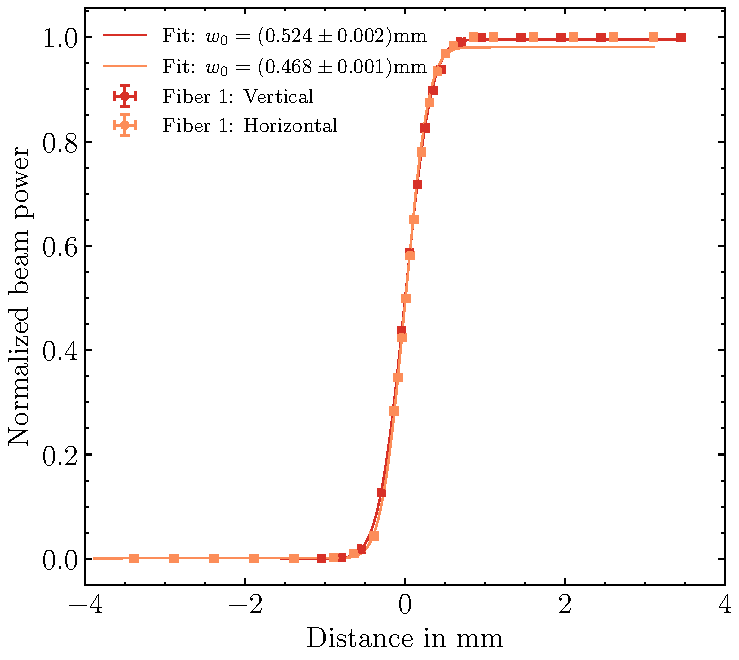
\includegraphics[width=1.\linewidth]{Fiber 1.pdf}
		\caption{Raman beam 1 (R1)}
		\label{fig:raman_beams_radius_1}
	\end{subfigure}%
	\begin{subfigure}{.5\textwidth}
		\centering
		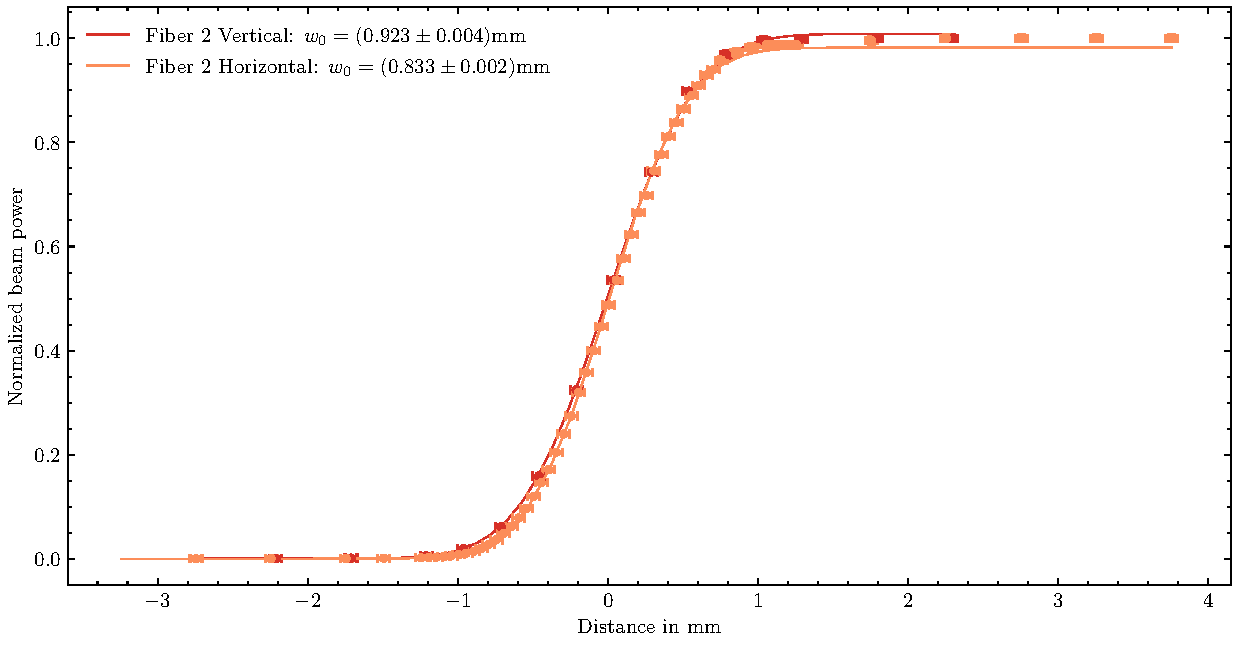
\includegraphics[width=0.955\linewidth]{Fiber 2.pdf}
		\caption{Raman beam 2 (R2)}
		\label{fig:raman_beams_radius_2}
	\end{subfigure}
	\caption[Beam radius measurement of the Raman beams performed with a knife-edge method]{Beam radius measurement of the Raman beams performed with a knife-edge method. The beam profile was measured at approximately the atomic cloud position. Each of the beams were measured in a vertical (red) and horizontal (orange) position.}
	\label{fig:raman_beams_radius}
\end{figure}


\section{Characterization of the \SI{841}{\nano\meter} erbium transition}

The following part consists in studying the \SI{841}{\nano\meter} erbium transition by blocking arbitrarily the beam R2 and allowing only R1 to interact with the erbium \ac{bec}. It is expected that the single running wave near resonance will heat the atoms, so that in this case the \ac{bec} population fraction reduces. After an interaction time of 10\si{\milli\second} in the final part of the evaporation phase, the atomic ensemble falls freely during a \ac{tof} of 20\si{\milli\second}. Then, the measurement is taken with the absorption imaging phase. From these measurements, the number of atoms can be estimated and the result, after scanning the frequency of R1, is shown in Figure \ref{fig:resonance_841_transition}. The data with a maximum of $N_\text{max} = 34849$ atoms was taken as normalization factor. As it can be seen from the image, the plot shows a drop in the atom number when the laser is locked to a wavelength of approximately \SI{840.98827}{\nano\meter} in air. This is because most of the atoms forming a \ac{bec} are resonant at this wavelength and get excited by the R1 beam, which expel them out of the ensemble and reduce drastically the atom number. In order to avoid effects like power broadening, the optical power of R1 has been kept as low as possible: $P_{\text{R1}} = (49.0 \pm 0.5) \si{\milli\watt}$. This way, the Gaussian fit performed in Figure \ref{fig:resonance_841_transition} gives an estimation of the resonant wavelength $\lambda_0^*$ and the linewidth $\Delta\nu_{\text{PB}}$ broadened mostly due to the beam power as
\begin{align*}
	\lambda_0^* &= 840.988266(2)\si{\nano\meter}   &   \Delta\nu_{\text{PB}} &= (3600 \pm 1700)\si{\kilo\hertz}
\end{align*}

The result is a quite accurate estimation of $\lambda_0^*$ while the calculation for $\Delta\nu_{\text{PB}}$ is not. The main reason is due to limitations in the scanning precision of the wave-meter, which was locking the laser. In any case, the measurement of $\Delta\nu_{\text{PB}}$ is helpful when comparing it to the theoretical linewidth of the transition $\Delta\nu_0 = \Gamma/2\pi = \SI{7.96}{\kilo\hertz}$ (see Table \ref{tab:Transitions}). Giving a real scenario of how big the one-photon detuning $\delta$ must be to make reasonable the approximations used for the Raman transition processes. On the other hand, the estimation of $\lambda_0^*$ contains a source of errors that has not been considered so far. This is the uncertainty coming from the laser frequency lock, which can not be assumed to remain constant and may shift during measurements. For this reason, the one-photon detuning $\delta$ estimation will be obtained with by using as resonance wavelength in air the following value:
\begin{equation*}
	\lambda_{0} = 840.98827(1)\si{\nano\meter}
\end{equation*}

\begin{figure}\centering
	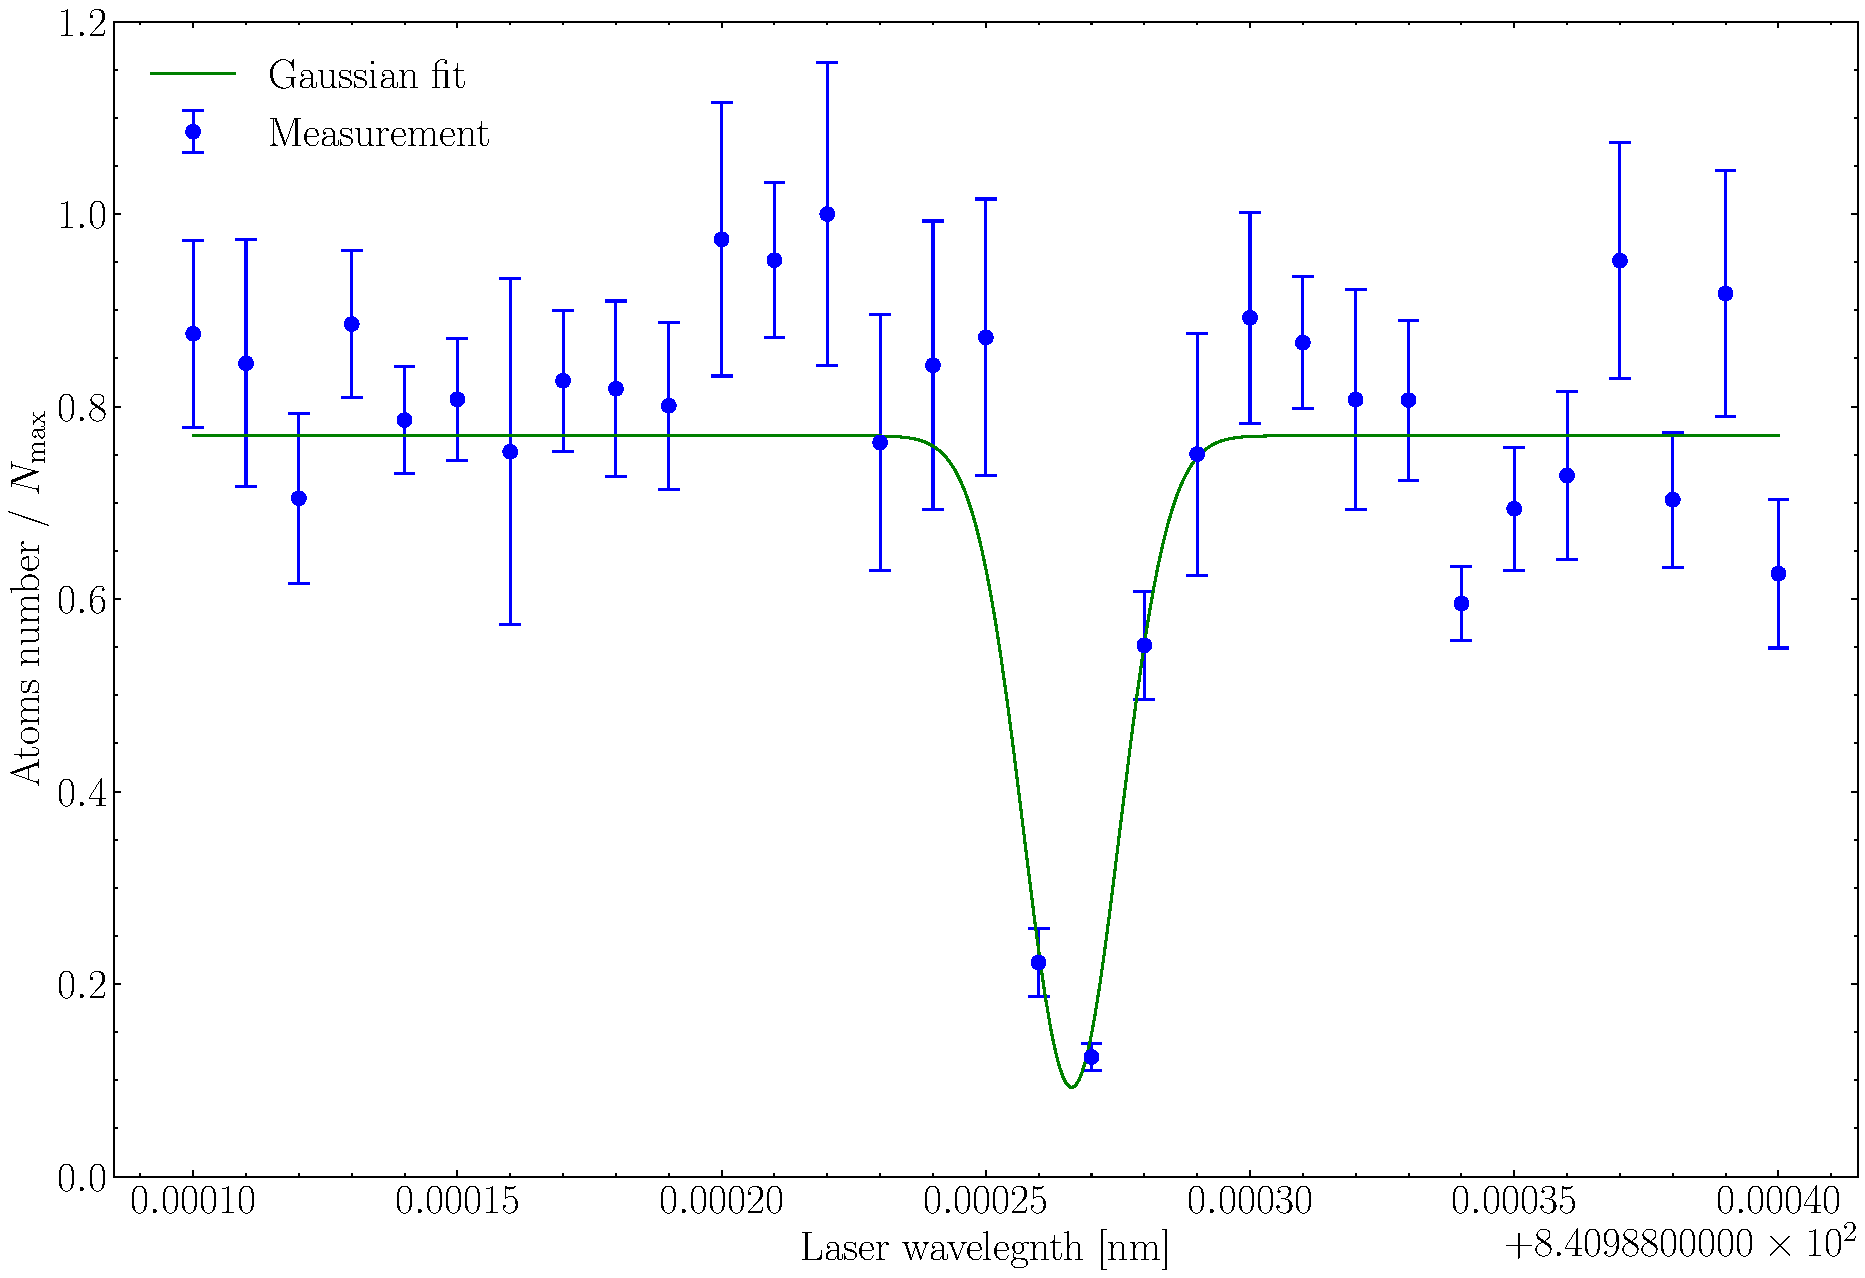
\includegraphics[width=1.\columnwidth]{Plot_resonance.pdf}
	\caption[Interaction of an erbium \ac{bec} with the beam R1]{Interaction of an erbium \ac{bec} with the beam R1. The plot shows the atom number of the \ac{bec} after a pulse of R1, normalized to the maximum measured value, as a function of the laser wavelength in air. The interaction between R1 and the atomic ensemble lasts 10\si{\milli\second} before the end of evaporation phase in every experimental cycle. Each measured point has been obtained by averaging the atom number of 5 experimental cycles. }\label{fig:resonance_841_transition}
\end{figure}

\section{Diffraction of an erbium \ac{bec} off a 1D-lattice potential}

Now, it is the moment to study the diffraction of an erbium \ac{bec} with the described Raman lattice set-up. In order to do this, the one photon detuning $\delta$ must be measured. Due to the conclusions made in previous section, the optical frequency of the Raman beams has been chosen for this whole part to be $\lambda_\text{R} = 840.98880(1) \si{\nano\meter}$. Thus, the resulting value for $\delta$ turns out to be
\begin{equation*}
	\delta = 2\pi c\cdot\bigg(\frac{1}{\lambda_{0}} - \frac{1}{\lambda_\text{R}} \bigg) = 2\pi \cdot(225 \pm 6) \si{\mega\hertz} \approx \num{1.8e5} \cdot\Delta\nu_0.
\end{equation*}

Therefore, the approximations used for the Hamiltonian in Section \ref{subsec:diffraction_regimes} are fulfilled. Because $\delta \gg \Gamma, \Delta\nu_0$ being the decay rate $\Gamma$ and natural linewidth $\Delta\nu_0$ of the \SI{841}{\nano\meter} transition (see Table \ref{tab:Transitions}). Another approximation that has been performed along this thesis results to be $\delta \gg \omega_r = \frac{\Delta_1}{4}$, with the 2-photon recoil frequency $\Delta_1$ given by Equation \eqref{eq:Bragg_condition} with $n=1$. From this expression one can get the value of $\Delta_1$ to be
\begin{equation*}
	\Delta_1 = \frac{2\hbar k^2}{M} = 2\pi \cdot (6.713 \pm 0.004)\si{kHz}.
\end{equation*}
This result proves the approximation $\delta \gg \Delta_1$ to also be reasonable within the described situation. Therefore, the different theoretical regimes seem to be valid and a more in-depth study is possible.

\subsection{Bragg regime}

As seen in Chapter \ref{chap:one_dimensional_lattices}, the Bragg regime is achieved only for long interaction times and when the Bragg condition is being fulfilled. To achieve it, the detuning between Raman beams has been set to $\Delta_1$. The result is an effective two level system between the 0th and +1st diffraction orders acting as ground and excited states respectively. This generates Rabi oscillations for different interaction times $t_\text{int}$ with frequency $\Omega_\text{eff}$ between the ground and excited state population rates, with the last one ideally governed by Equation \ref{eq:population_excited_state}. This effect has been observed for the case of optical power in the Raman beams chosen like: $P_1 = (3.05 \pm 0.05)\si{\milli\watt}$ and $P_2 = (9.10 \pm 0.05)\si{\milli\watt}$. These powers allow to estimate the ``effective'' average intensity of the standing wave as
\begin{equation*}
	I_\text{eff} = \sqrt{I_1\cdot I_2} = (7.7 \pm 0.4)\si{\kilo\watt\per\meter\squared}.
\end{equation*} 

Figure \ref{fig:Bragg_images} shows the effect of Rabi oscillations between the 0th and 1st orders for the exposed value of $I_\text{eff}$. These images are just a small sample of all the measured for this same situation but different values of $t_\text{int}$. From each image, the relative population of any $i$ order with $i \in \{0,1\}$ can be estimated as
\begin{equation}
	P_i = \frac{N_i}{N_0+N_1},
\end{equation}
where $N_0$ and $N_1$ are the number of atoms in each diffraction order. Therefore, it is possible to measure the relative population in each picture and plot it as a function of $t_\text{int}$. This is shown in Figure \ref{fig:Bragg_measurement}.

\begin{figure}[!htbp]
	\centering
	\begin{subfigure}{.33\textwidth}
		\centering
		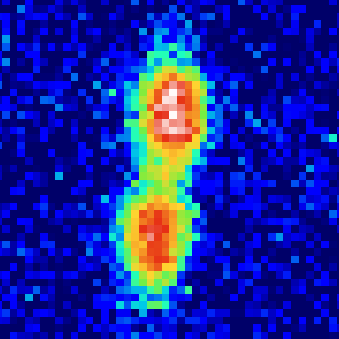
\includegraphics[width=.9\linewidth]{Rabi_measurement_60us.png}
		\caption{ $t_\text{int} = 60\si{\micro\second}$}
		\label{fig:Bragg_images_1}
	\end{subfigure}%
	\begin{subfigure}{.33\textwidth}
		\centering
		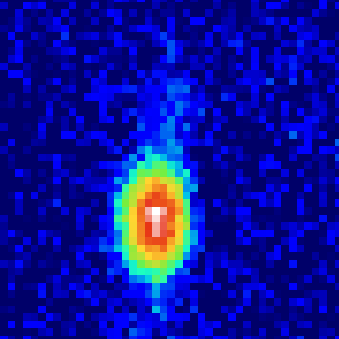
\includegraphics[width=.9\linewidth]{Rabi_measurement_120us.png}
		\caption{ $t_\text{int} = 120\si{\micro\second}$}
		\label{fig:Bragg_images_2}
	\end{subfigure}
	\begin{subfigure}{.33\textwidth}
		\centering
		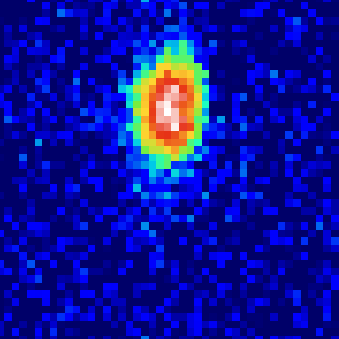
\includegraphics[width=0.9\linewidth]{Rabi_measurement_240us.png}
		\caption{ $t_\text{int} = 240\si{\micro\second}$}
		\label{fig:Bragg_images_3}
	\end{subfigure}
	\caption[Diffracted ultracold erbium ensemble after an interaction time with the lattice $t_\text{int}$ and a \ac{tof}$=19\si{\milli\second}$]{Diffracted ultracold erbium ensemble after an interaction time with the lattice $t_\text{int}$ and a \ac{tof}$=19\si{\milli\second}$. One can observe the effect of Rabi oscillations due to different $t_\text{int}$ values. The top atomic cloud corresponds to the 0th diffraction order while the bottom cloud is the 1st. Each image has been normalized with respect to the maximum and minimum value in the frame. The used camera is rotated 90° counter-clockwise, resulting in the separation of orders in the vertical axis of the frames. The effective intensity of the lattice used was $I_\text{eff} = (7.7 \pm 0.4)\si{\kilo\watt\per\meter\squared}$.}
	\label{fig:Bragg_images}
\end{figure}

\begin{figure}[!htbp]\centering
	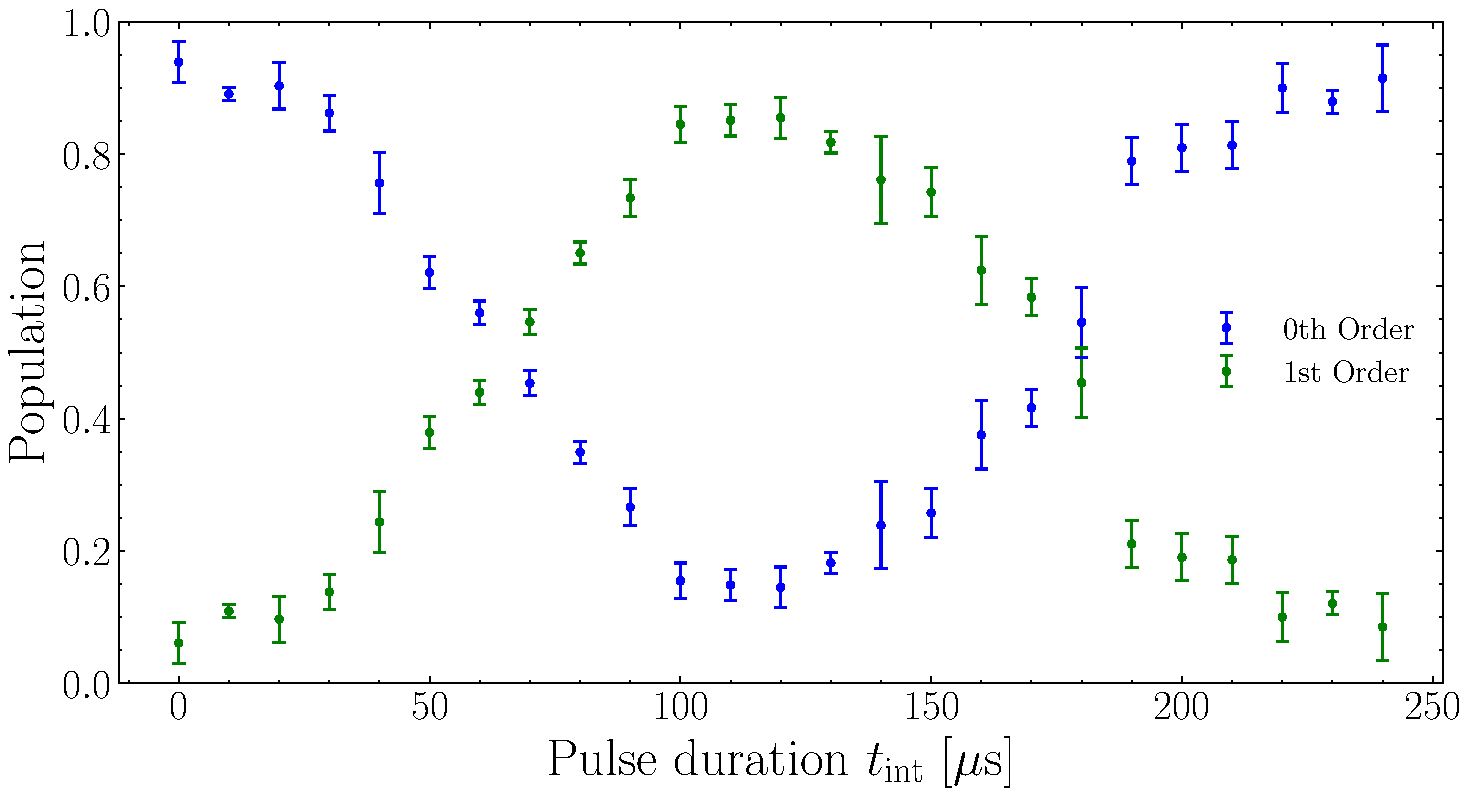
\includegraphics[width=1.\columnwidth]{Rabi_measurement_7.7.pdf}
	\caption[Relative population as a function of the interaction time between erbium \ac{bec} and Raman lattice]{Relative population as a function of the interaction time between erbium \ac{bec} and Raman lattice. The plot shows Rabi oscillations in populations of the 0th and 1st diffraction orders. Each pair of points has been taken by averaging 5 different images. The Raman lattice had an effective average intensity of $I_\text{eff} = (7.7 \pm 0.4)\si{\kilo\watt\per\meter\squared}$. }\label{fig:Bragg_measurement}
\end{figure}

The plot confirms the theory and shows Rabi oscillations in an effective 2-level system as a predominant effect for this regime of parameters. Once this set of data is obtained, one can perform a more in-depth analysis of the oscillations. As it has been said, Equation \ref{eq:population_excited_state} must be fulfilled in this regime for the behaviour of population in the 1st diffracted order $P_1$. This way, a sine squared function fit can be performed to this population rate. However, in order to account for factors like noise or coherent losses in the \ac{bec}, a damped term has been added. Thus, the fitted function expression results
\begin{equation}
	f_\text{fit}(t_\text{int}) = A \text{exp}(-b t_\text{int}) \cdot \text{sin}^2\bigg(\frac{\Omega_\text{eff}t_\text{int}}{2} +\phi\bigg) + y_0,
\end{equation}
where $A$, $b$, $\Omega_\text{eff}$, $\phi$ and $y_0$ are free parameters of the fit. This allows the estimation of relevant system parameters such as the 2-photon Rabi frequency for any value of $I_\text{eff}$. The result can be seen in Figure \ref{fig:Bragg_fit_1st_order} for three different values of $I_\text{eff}$. From this analysis, one can easily see a proportional relation between $I_\text{eff}$ and $\Omega_\text{eff}$, which is also described in the theory. When combining Equations \eqref{eq:relation_rabi_frequency_lattice_depth} and \eqref{eq:relation_lattice_potential_depth_final} one gets
\begin{equation}\label{eq:relation_Ieff_omega_eff}
	\Omega_\text{eff} = \Bigg(\frac{3 \pi c^2 \Gamma}{\omega_0^3 \delta \hbar} \text{exp}\bigg(-\frac{r_1^2}{w_1^2}-\frac{r_2^2}{w_2^2}\bigg)\Bigg) \cdot I_\text{eff},
\end{equation}
which contains an exponential term describing how ``good'' the Raman beams are aligned with respect to the erbium \ac{bec}. Unfortunately, this term can not be measured independently within a reasonable value of uncertainty. However, it can be estimated with the obtained data by simply performing a linear fit to the measured values of $\Omega_\text{eff}$ as a function of $I_\text{eff}$. This can be seen in Figure \ref{fig:Linear_fit}.


\begin{figure}[!htbp]
	\centering
	\begin{subfigure}{1.\textwidth}
		\centering
		\label{fig:fig:Bragg_fit_1st_order_7.7}
		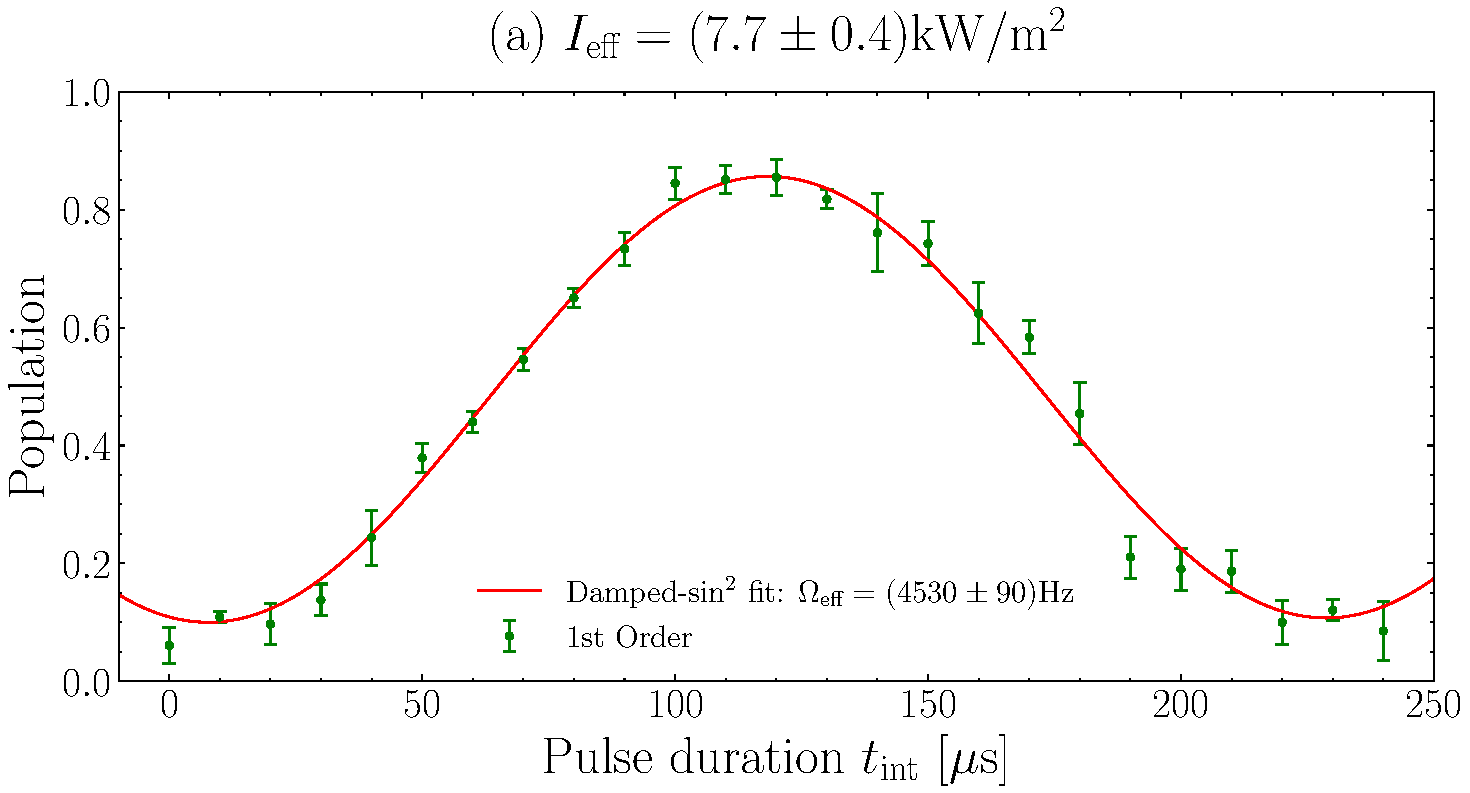
\includegraphics[width=.8\linewidth]{Rabi_fit_7.7.pdf}
		%\caption{$I_\text{eff} = (7.7\pm 0.4)\si{\kilo\watt\per\meter\squared}$}
	\end{subfigure}%
	\hfill
	\vspace{0.2cm}
	\begin{subfigure}{1.\textwidth}
		\centering
		\label{fig:Bragg_fit_1st_order_12.7}
		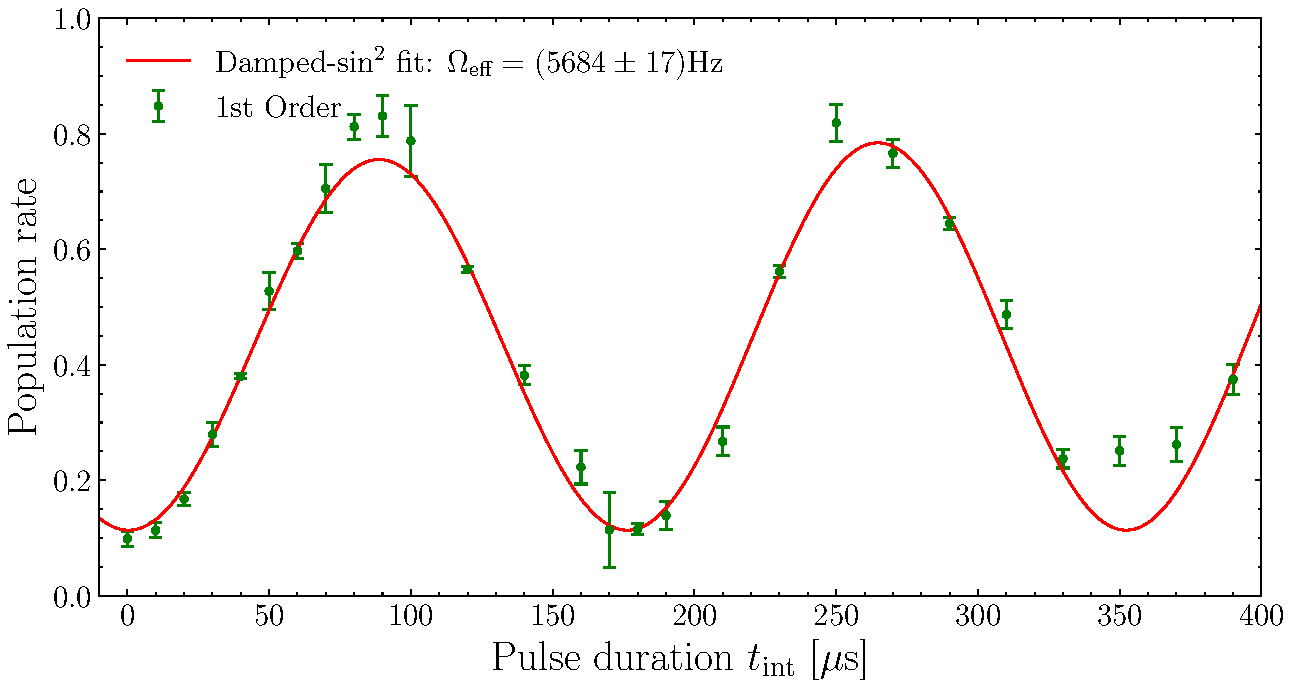
\includegraphics[width=.8\linewidth]{Rabi_fit_12.7.pdf}
		%\caption{$I_\text{eff} = (12.7\pm 0.4)\si{\kilo\watt\per\meter\squared}$}
	\end{subfigure}
	\hfill
	\vspace{0.2cm}
	\begin{subfigure}{1.\textwidth}
		\centering
		\label{fig:Bragg_fit_1st_order_24.6}
		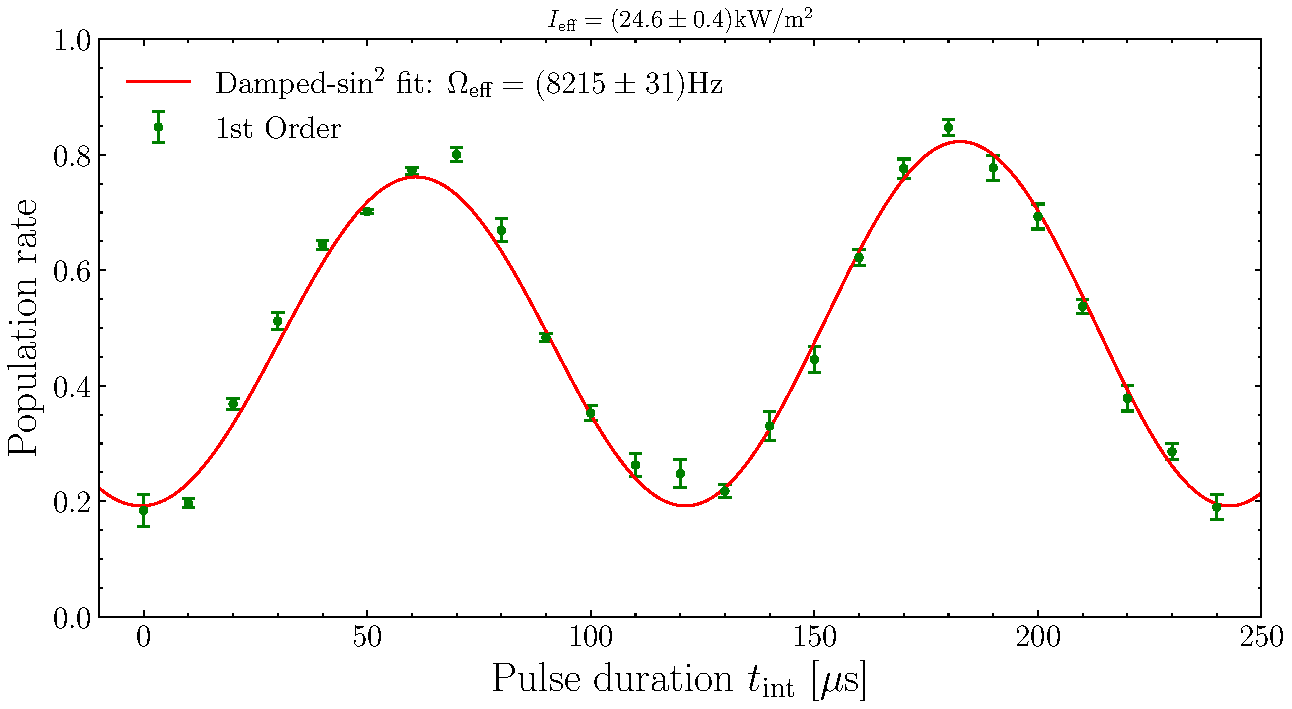
\includegraphics[width=0.8\linewidth]{Rabi_fit_24.6.pdf}
		%\caption{$I_\text{eff} = (24.6\pm 0.4)\si{\kilo\watt\per\meter\squared}$}
	\end{subfigure}
	\caption[Fit of a damped sine squared function to the population rate for different values of $I_\text{eff}$]{Fit of a damped sine squared function to the population rate for different values of $I_\text{eff}$. The objective is to characterize the Rabi oscillations in this state and obtain an estimation of the 2-photon Rabi frequency $\Omega_\text{eff}$.}
	\label{fig:Bragg_fit_1st_order}
\end{figure}

\begin{figure}[!htbp]\centering
	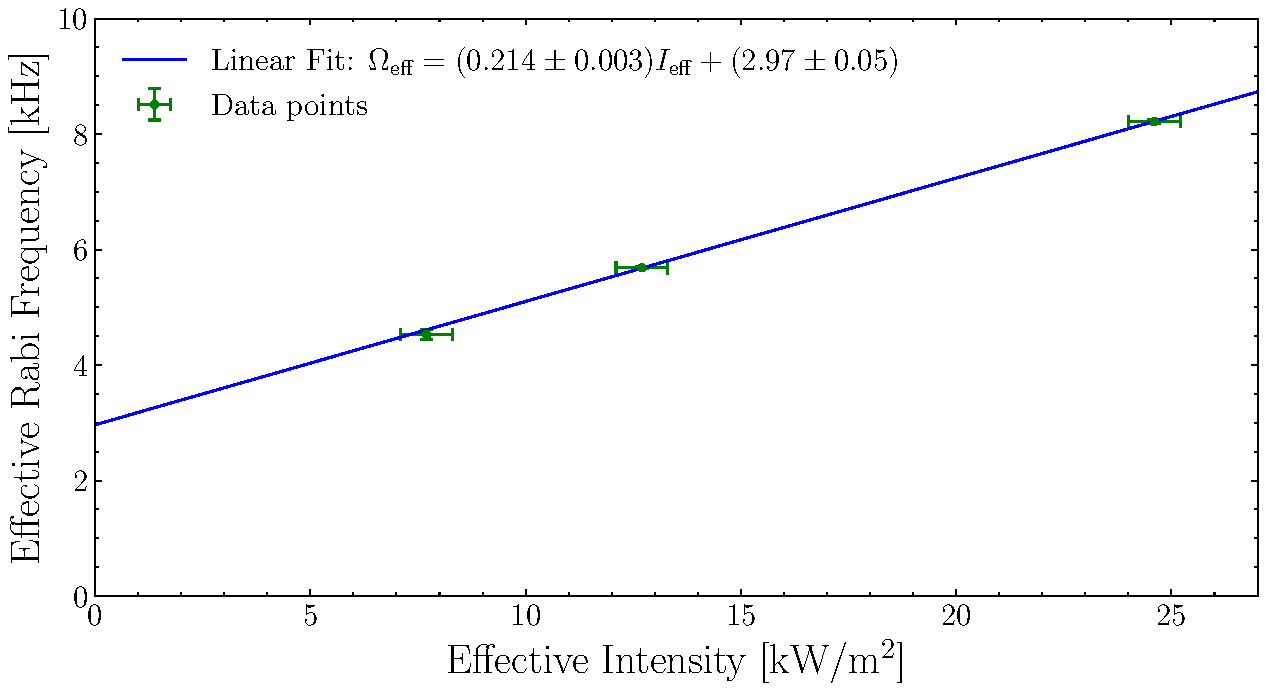
\includegraphics[width=1.\columnwidth]{Linear_Fit.pdf}
	\caption[Linear fit of the 2-photon Rabi frequency as a function of the effective intensity in the lattice]{Linear fit of the 2-photon Rabi frequency as a function of the effective intensity in the lattice.}\label{fig:Linear_fit}
\end{figure}

\newpage

As a result, the linear fit seems to fulfil the measured data behaviour, which also coincides with theory. One could argue, the amount of data points to not be high enough. This is due to time constrains at the moment of taking the data, as different experimental problems appeared together with the requirement of measuring more data that will be shown below. In any case, the linear fit also shows a discrepancy with Equation \eqref{eq:relation_Ieff_omega_eff}, which consist in a non-zero intercept of $(2.97\pm0.05)\si{\kilo\hertz}$. This can be due to different reasons, the main one being the differences between Raman beam sizes. It could be a mayor factor because together with the beam misalignment, there will be a major difference between the optical intensities perceived by the \ac{bec}. This produces a shift in the lattice potential, which in principle should not affect these measurements for small shift values, but in the case of very big ones it could be a responsible factor. Other possibility is that the little amount of points covers a non-linear behaviour for small values of $I_\text{eff}$ for unknown reasons. 

In any case, the slope value of the linear fit is $(0.214\pm0.003)\si{\kilo\hertz\meter\squared\per\kilo\watt}$, which allows to compare it with theory and a perfect beam alignment ($r_1 = r_0 = 0$) at Equation \eqref{eq:relation_Ieff_omega_eff}. The obtained result is roughly two orders of magnitude below the theoretical expectation. The main source of this mismatch has already been discussed and corresponds to the misalignment of the Raman beams, forming the one-dimensional standing wave, with respect to the \ac{bec} position. As it has been shown, any displacement of the Raman beams from the \ac{bec} centre would result in an exponential decrease in the Rabi frequency and lattice depth parameters. This fact makes it the main contributing factor of the mismatch, but it could not be the only one. Other effect to have into account is the notable size difference between beams, which could lead to big differences in the perceived intensities by the \ac{bec} and could diminish the Rabi oscillation process. Another possibility is an error in the detuning estimation with respect to the atomic transition of erbium near \SI{401}{\nano\meter}, which is less likely but possible due to a shift in the laser frequency during the measurement.

\pagebreak

\subsection{Raman-Nath regime}

Once, the Bragg regime has been characterized, it is the moment of briefly showing that the Raman-Nath regime is also achievable in this experimental set-up. After ramping up the effective intensity in the optical lattice to $I_\text{eff} = (42.12 \pm 0.5)\si{\kilo\watt\per\meter\squared}$, and setting the 2-photon detuning between R1 and R2 to zero. The result can be seen in Figures \ref{fig:raman_nath} and \ref{fig:raman_nath_cut}, where an average of over 104 different pictures has been performed. As it can be seen, up to 5 different diffraction orders can be distinguished, which confirms the described theory and shows the experimental set-up capability to achieve the Raman-Nath regime.

\begin{figure}[!htbp]\centering
	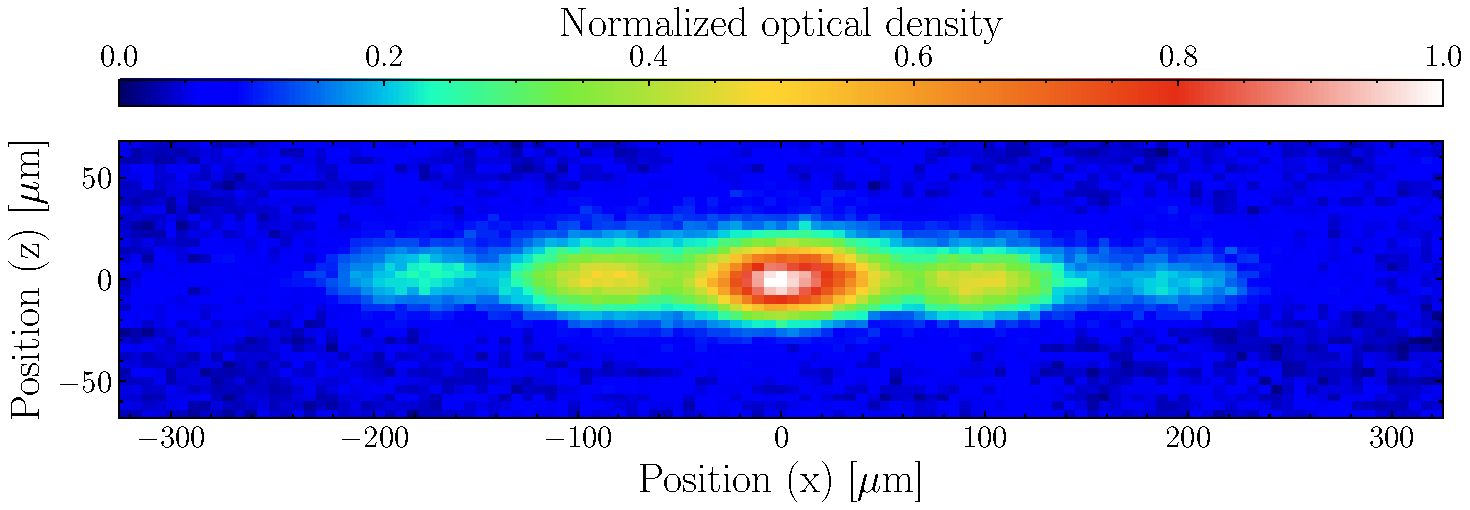
\includegraphics[width=1.\columnwidth]{raman_nath.pdf}
	\caption[Absorption image of a multiple orders diffracted \ac{bec} after a \ac{tof} of \SI{19}{\milli\second}]{Absorption image of a multiple orders diffracted \ac{bec} after a \ac{tof} of \SI{19}{\milli\second}. The result was obtained after an average of over 104 different pictures with an effective intensity of $I_\text{eff} = (42.12 \pm 0.5)\si{\kilo\watt\per\meter\squared}$. The image has been rotated to match the gravitational axis with the up-down axis in the frame.}\label{fig:raman_nath_cut}\label{fig:raman_nath}
\end{figure}

\begin{figure}[!htbp]\centering
	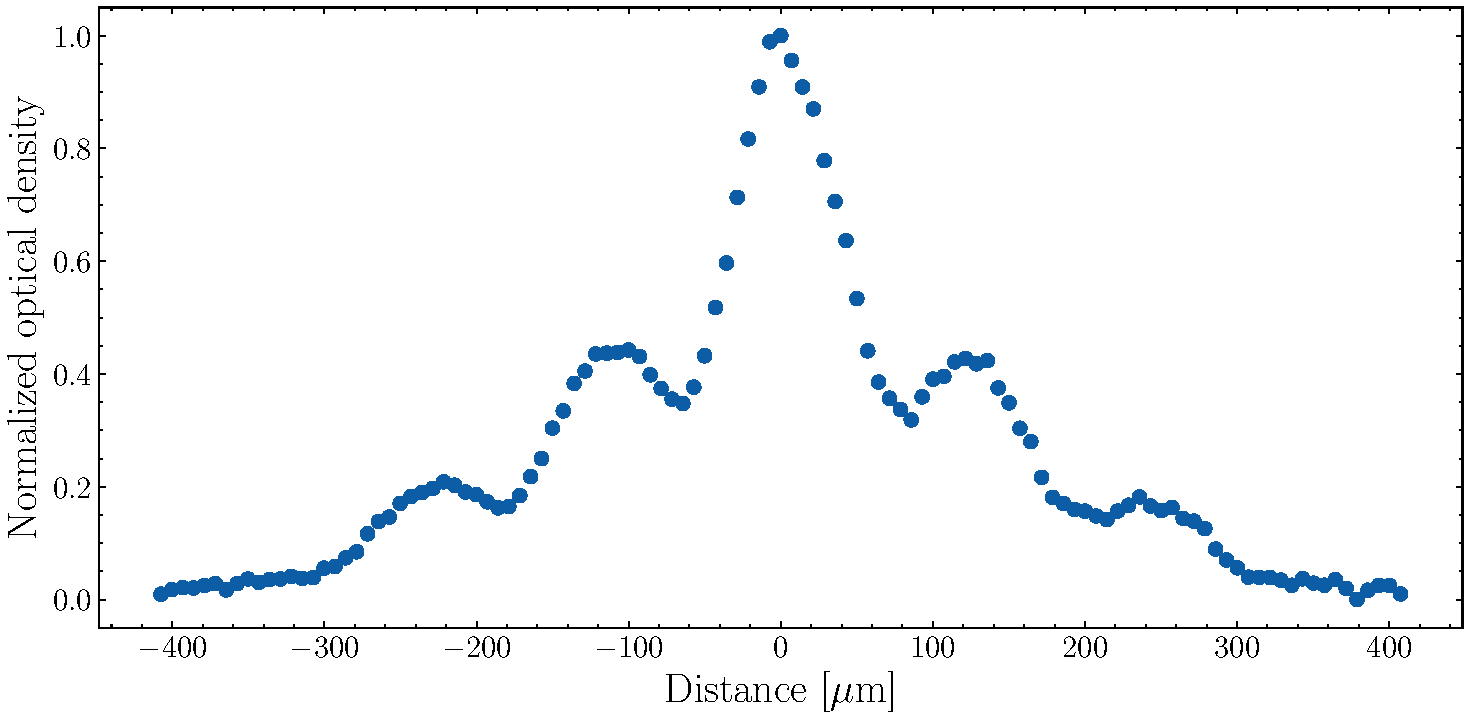
\includegraphics[width=1.\columnwidth]{raman_nath_cut.pdf}
	\caption[Average cut performed to the image shown in Figure \ref{fig:raman_nath}]{Average cut performed to the image shown in Figure \ref{fig:raman_nath}}
\end{figure}

\pagebreak

\section{Magnetic fields characterization with \acs{rf} transitions}

After characterising an optical set-up that results in Raman transitions between components in the momentum space, the following goal is already described in Chapter \ref{chap:raman_manipulation}. This objective consists in obtaining Raman transitions between components in the spin and momentum space. But first, it is required the use of \ac{rf} transitions to estimate the Zeeman splitting caused by the magnetic fields inside the vacuum chamber. This way, the effect can be compensated first and then an extra field can be added along the quantization axis of the Raman beams, which will be required for the Raman transitions. Section \ref{sec:rf_transitions} describes this in further detail, while here the focus will be in analysing the measured data. Figure \ref{fig:RF_pulse} shows two reference samples of the measurements. An erbium \ac{bec} interacts with an \ac{rf}-pulse during \SI{0.4}{\milli\second} and falls through a gradient field of approximately 4G/cm during the \ac{tof} of \SI{19}{\milli\second}, which allows the separation between Zeeman states due to the Stern-Gerlach force. When the \ac{rf}-pulse frequency is far away from the Zeeman resonance $\omega_\text{Ze} \equiv \Delta E_{\text{Ze}}/\hbar$ given by Equation \ref{eq:Zeeman_splitting_difference}, the result is shown in Figure \ref{fig:RF_pulse_non-resonant}. The \ac{rf} transitions are being suppressed and the \ac{bec} remains mostly in the state $m_J=-6$ due to the experimental set-up configuration (see Section \ref{sec:rf_transitions}). On the other hand, when the \ac{rf}-pulse frequency is close to $\omega_\text{Ze}$, the transitions into other Zeeman levels are allowed, as shown in Figure \ref{fig:RF_pulse_resonant}. Therefore, by scanning the \ac{rf}-pulse frequency in the region of Zeeman resonance and comparing the population in different states, one can get an estimation of $\omega_\text{Ze}$ produced by any homogeneous magnetic field $\vec{B}_\text{H}$. Thus, the measurements of $\omega_\text{Ze}$ for three different homogeneous fields can be seen in Figure \ref{fig:Plot_RF_All_fields}.

\begin{figure}[!htbp]
	\centering
	\begin{subfigure}{.5\textwidth}
		\centering
		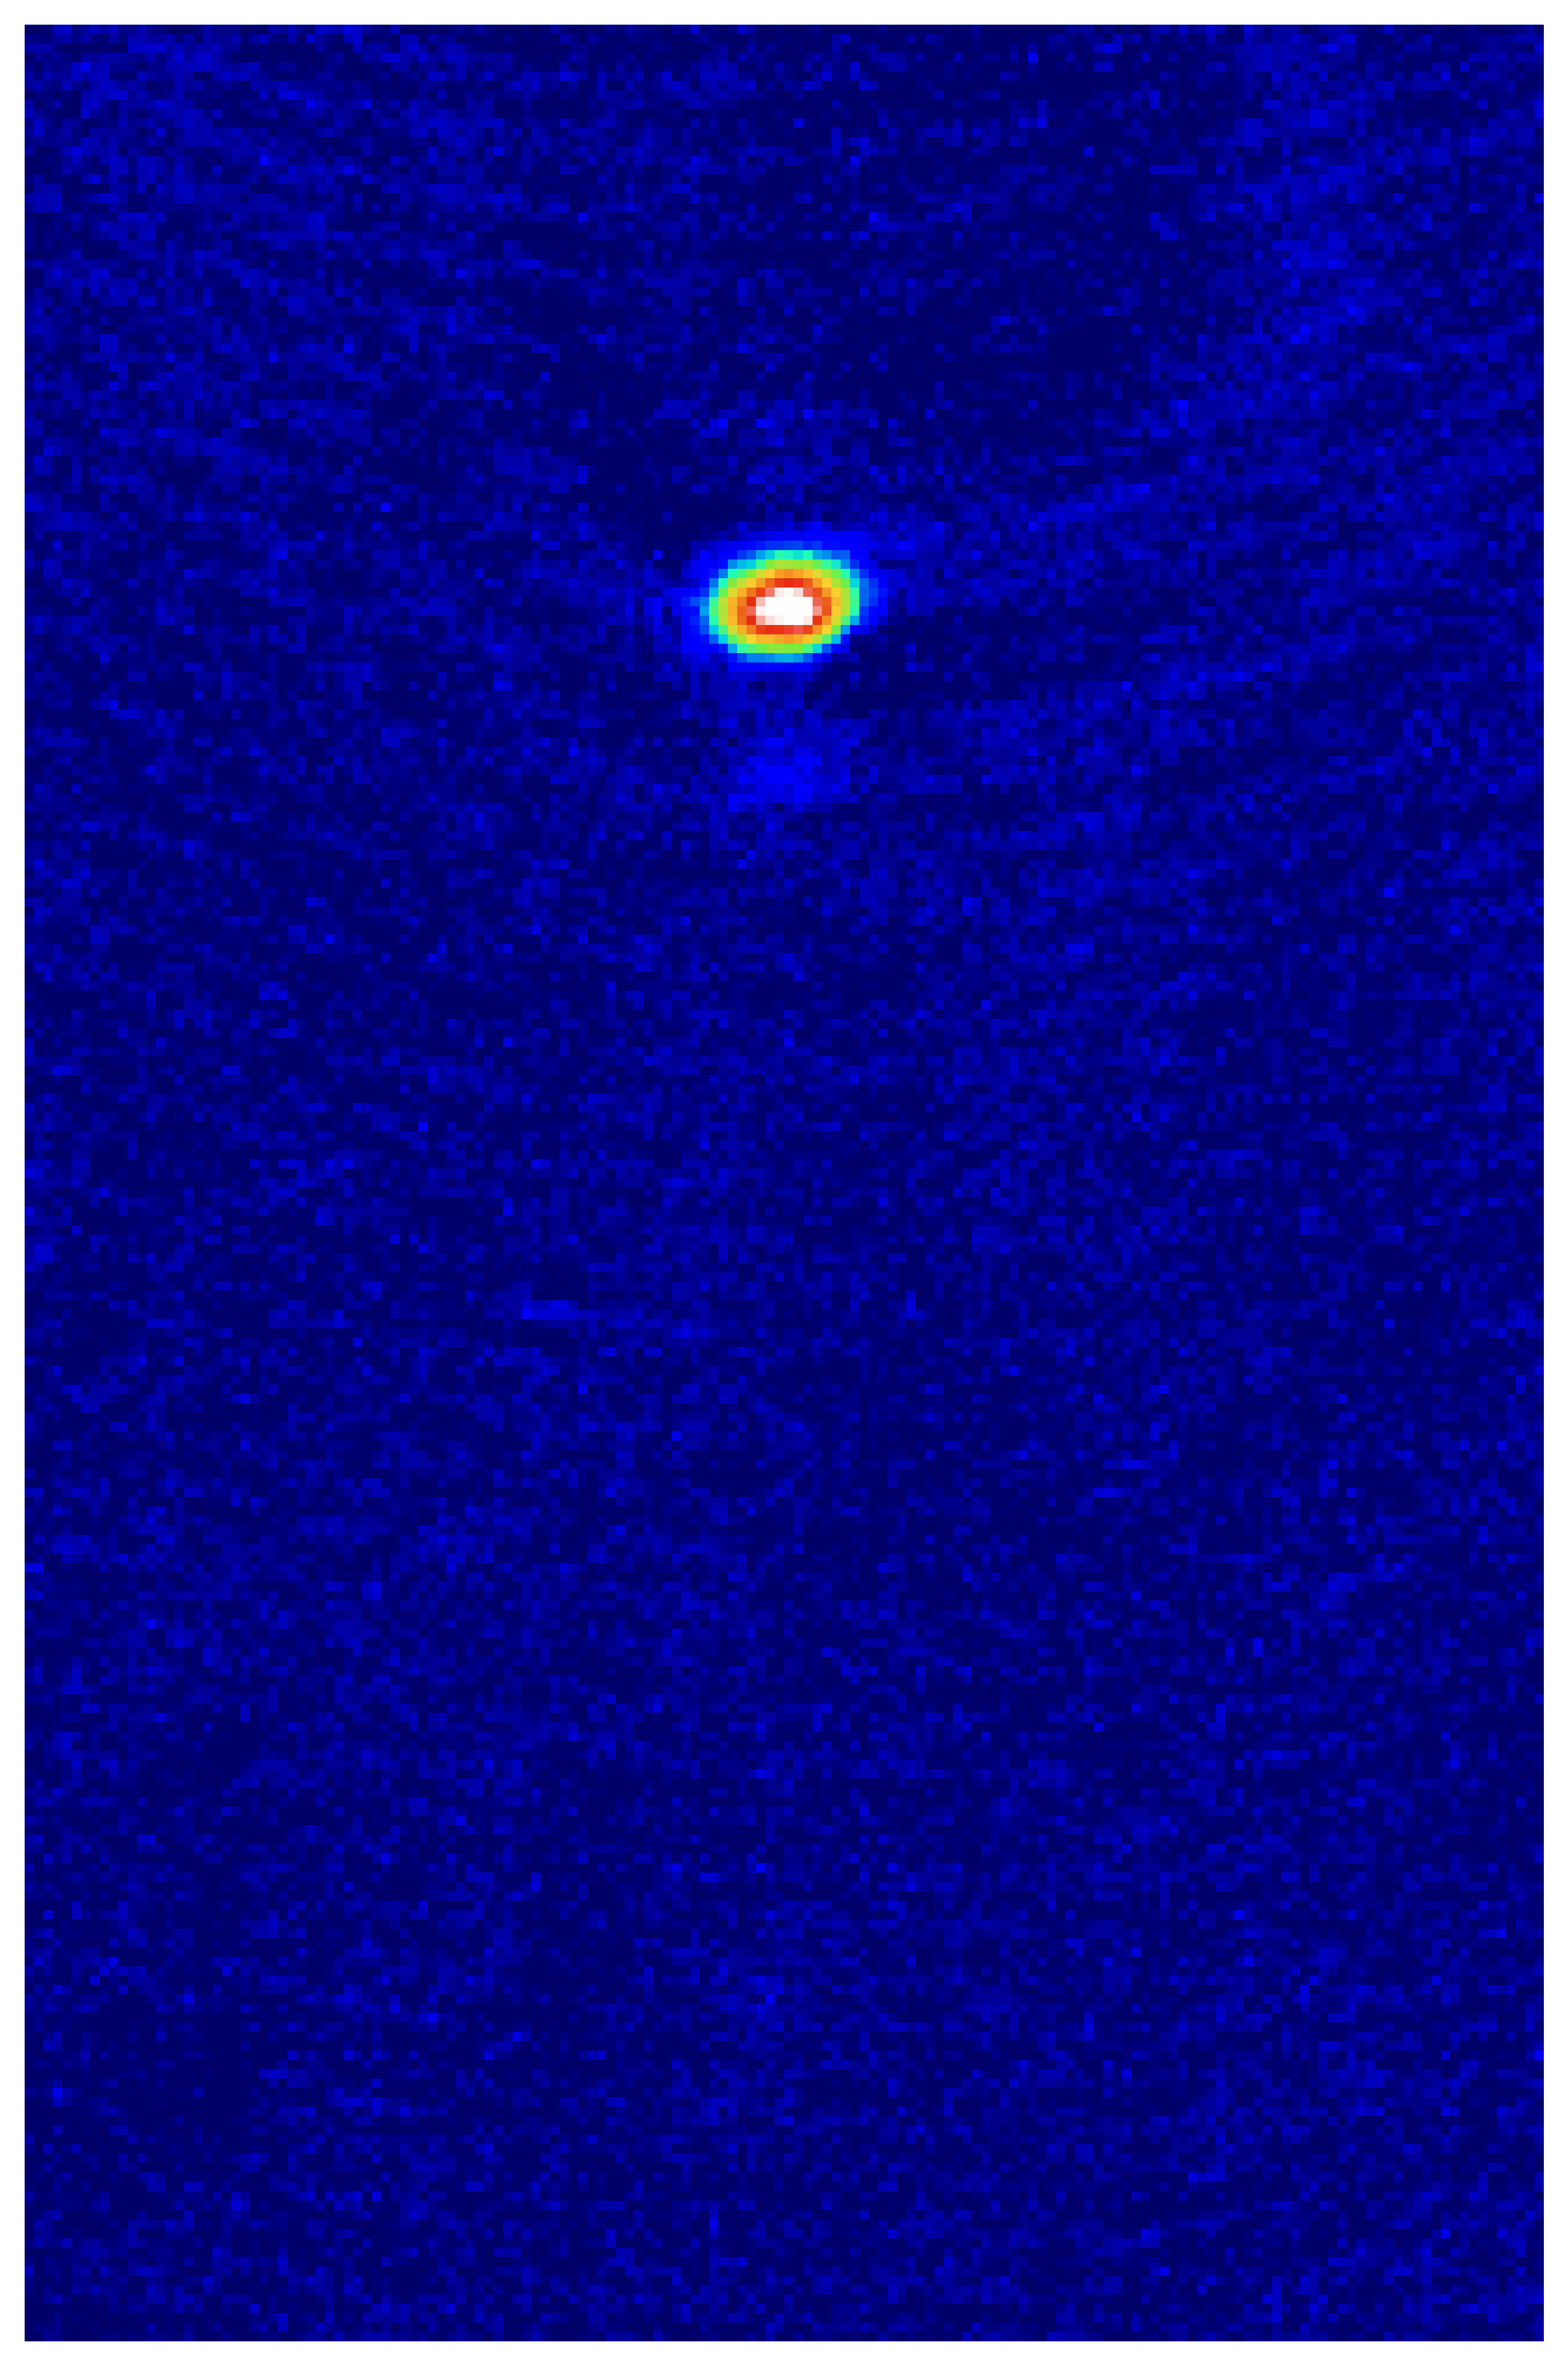
\includegraphics[width=0.7\linewidth]{RF_pulse_non-resonant.png}
		\caption{Far-resonant \ac{rf} pulse}
		\label{fig:RF_pulse_non-resonant}
	\end{subfigure}%
	\begin{subfigure}{.5\textwidth}
		\centering
		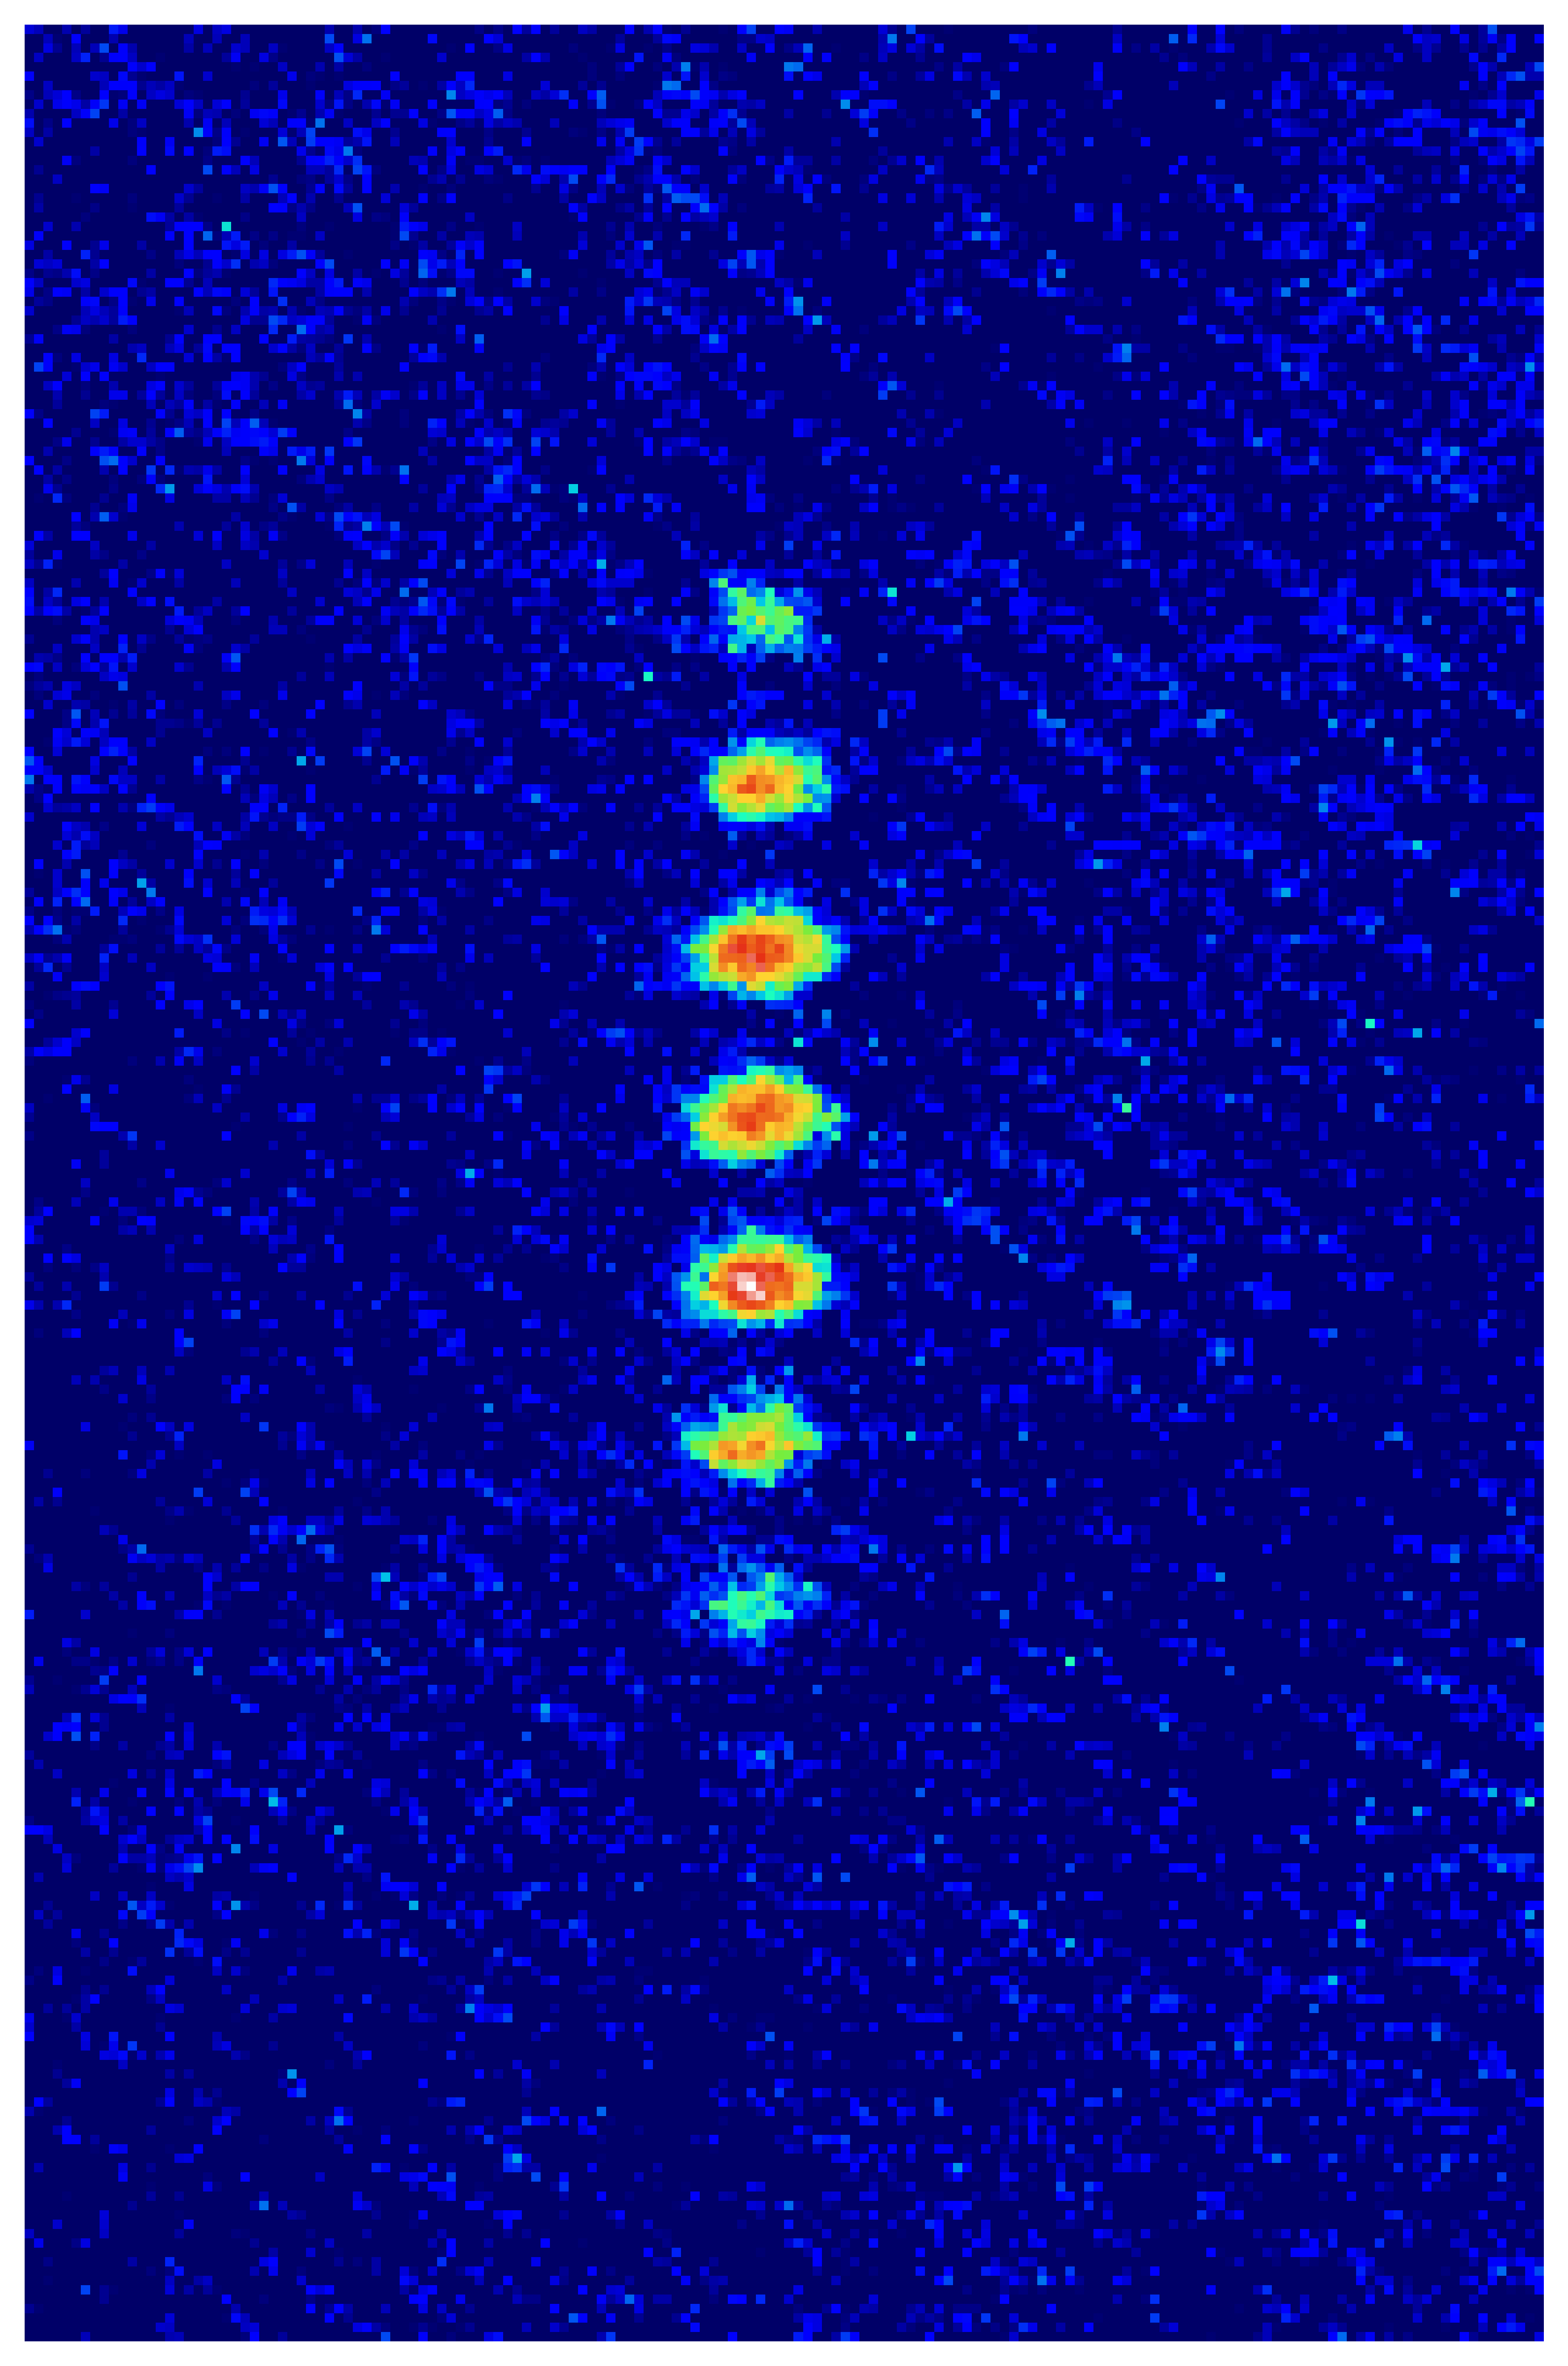
\includegraphics[width=0.7\linewidth]{RF_pulse_resonant.png}
		\caption{Near-resonant \ac{rf} pulse}
		\label{fig:RF_pulse_resonant}
	\end{subfigure}
	\caption[Comparative set of two different interactions between an erbium \ac{bec} and a \ac{rf}-pulse.]{Comparative set of two different interactions between an erbium \ac{bec} and a \ac{rf}-pulse. Both images were taken after an interaction time with the \ac{rf}-pulse of \SI{0.4}{\milli\second} and a \ac{tof} of \SI{19}{\milli\second}. During this \acl{tof} a gradient field of approximately 4G/cm was applied in order to separate the different $m_J$ orders. The gradient field direction was being applied along the gravitational axis, which corresponds to the vertical direction in both images.}
	\label{fig:RF_pulse}
\end{figure}



\begin{figure}[!htbp]
	\centering
	\begin{subfigure}{1.\textwidth}
		\centering
		\label{fig:Plot_RF_Experiment_fields}
		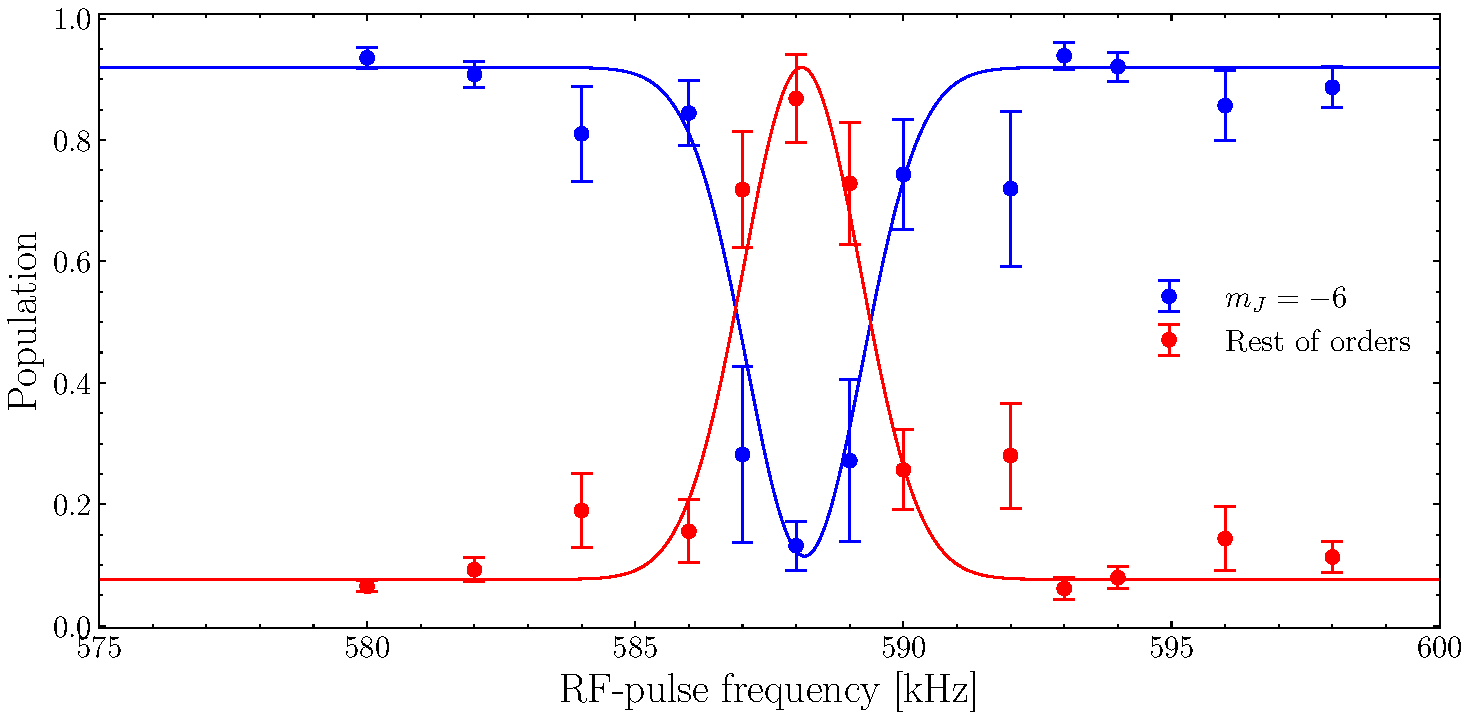
\includegraphics[width=.75\linewidth]{Plot_RF_Experiment_fields.pdf}
		\caption{Experiment magnetic field $\vec{B}_\text{H}$}
	\end{subfigure}%
	\hfill
	\vspace{0.2cm}
	\begin{subfigure}{1.\textwidth}
		\centering
		\label{fig:Plot_RF_Compensated_fields}
		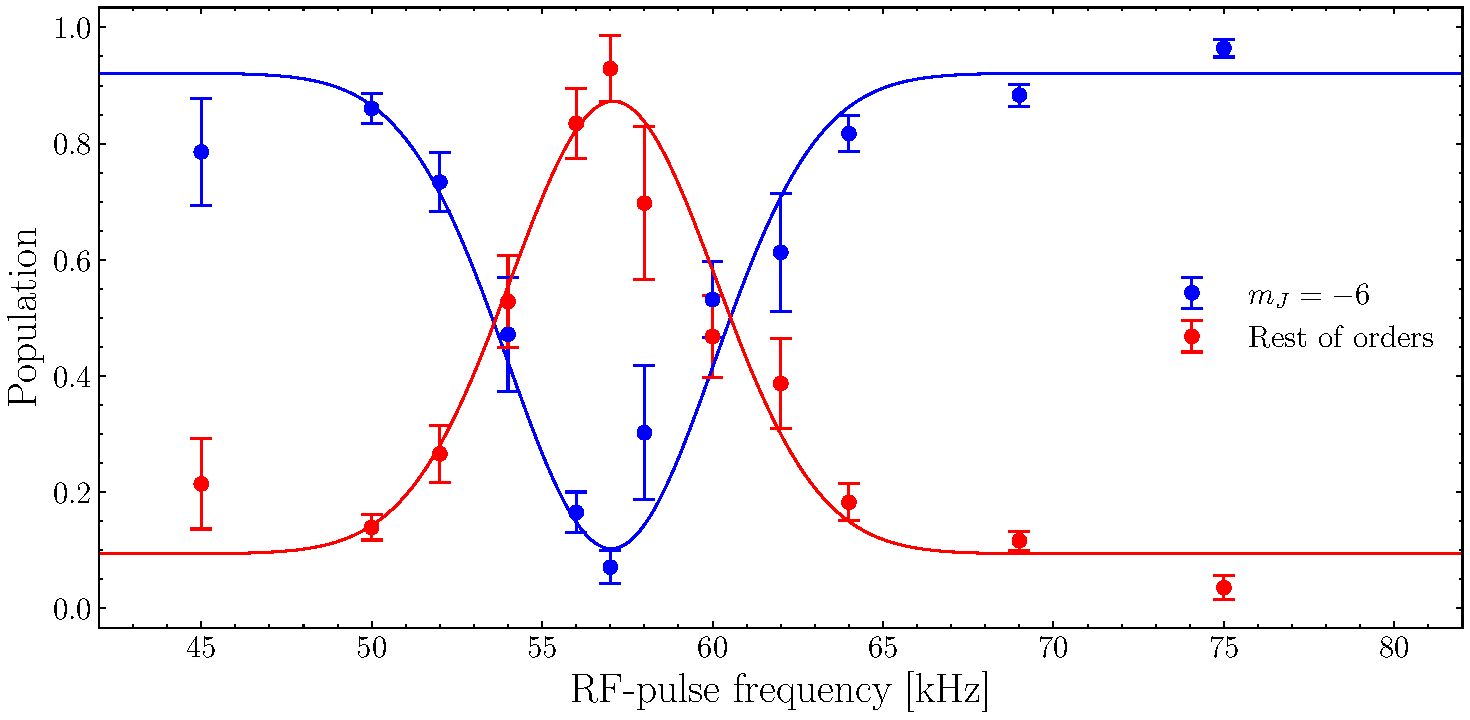
\includegraphics[width=.75\linewidth]{Plot_RF_Compensated_fields.pdf}
		\caption{Compensated magnetic field $\vec{B}_\text{Comp}$}
	\end{subfigure}
	\hfill
	\vspace{0.2cm}
	\begin{subfigure}{1.\textwidth}
		\centering
		\label{fig:Plot_RF_Known_fields}
		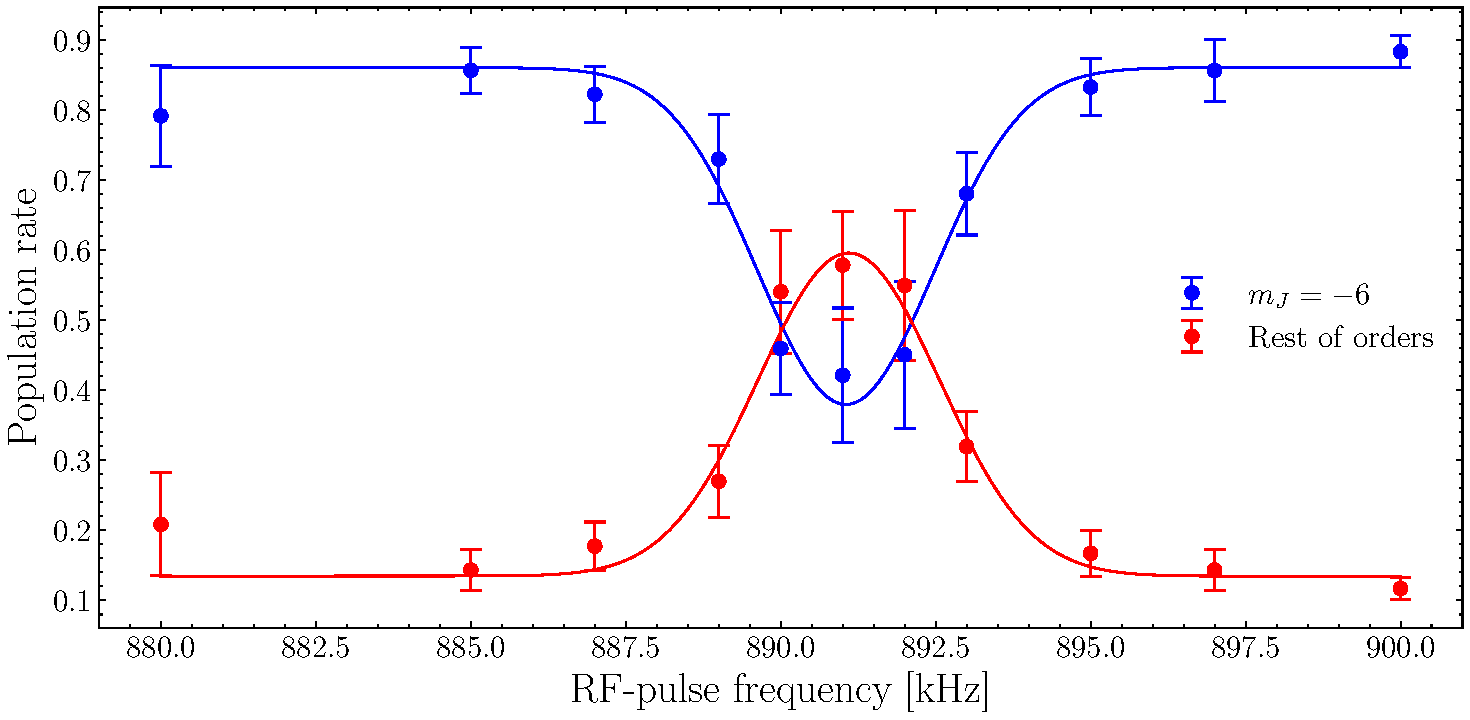
\includegraphics[width=0.75\linewidth]{Plot_RF_Known_fields.pdf}
		\caption{Added magnetic field $\vec{B}'_\text{H} = \vec{B}_\text{Comp} +B_\text{R}\vec{e}_x$}
	\end{subfigure}
	\caption[Measured frequency spectrum of the \ac{rf} transitions for different homogeneous magnetic fields causing the splitting of Zeeman states in the erbium \ac{bec}]{Measured frequency spectrum of the \ac{rf} transitions for different homogeneous magnetic fields causing the splitting of Zeeman states in the erbium \ac{bec}. This data has been obtained measuring the population in each state and comparing the result for state $m_J = -6$ with the added population of the rest $m_J = $-5, -4, ..., +6. A Gaussian fit has been applied in each set of data in order to obtain an estimation of the resonant frequencies and transition linewidths.}
	\label{fig:Plot_RF_All_fields}
\end{figure}

\pagebreak

Each plotted data in the three parts of Figure \ref{fig:Plot_RF_All_fields} corresponds to a ratio of the atom number in the ground state $m_J = -6$ and the rest of states $m_J = $-5, -4, ..., +6. The different fields are: $\vec{B}_\text{H}$ the default magnetic field affecting the \ac{bec} during the experiment, $\vec{B}_\text{Comp}$ the compensated field with offset coils in order to make $\omega_\text{Ze}$ as low as possible, and $\vec{B}'_\text{H} = \vec{B}_\text{Comp} +B_\text{R}\vec{e}_x$ the result of adding to the compensated field and extra one in the Raman beams direction for the following section. By applying a Gaussian fit to each set of data, an estimation of relevant parameters like the Zeeman resonant frequencies $\omega_\text{Ze}$ and the \ac{rf} transition linewidths $\Delta \omega_\text{Ze}$ were obtained:

\begin{table}[htbp] \centering
	\begin{tabular}{@{}l|c|c@{}}\hline
	Magnetic field	                  & $\omega_\text{Ze} [\si{\kilo\hertz}]$           & $\Delta \omega_\text{Ze} [\si{\kilo\hertz}]$ \\ \hline\hline
	$\vec{B}_\text{H}$	     &  $588.1 \pm 0.1 $   & $1.1 \pm 0.4 $        \\
	$\vec{B}_\text{Comp}$	 &  $57.06 \pm 0.15 $  & $3.0 \pm 0.9 $        \\ 
	$\vec{B}'_\text{H}$	     &  $891.08 \pm 0.14 $ & $1.4 \pm 0.7 $       \\\hline
	\end{tabular}
	\caption[Estimation of the Zeeman resonant frequencies $\omega_\text{Ze}$ and the \ac{rf} transition linewidths $\Delta \omega_\text{Ze}$]{Estimation of the Zeeman resonant frequencies $\omega_\text{Ze}$ and the \ac{rf} transition linewidths $\Delta \omega_\text{Ze}$ from the Gaussian fits performed in Figure \ref{fig:Plot_RF_All_fields}.}
	\label{tab:results_Plot_RF_All_fields}
\end{table}

These results are reasonable and for the case of $\Delta \omega_\text{Ze}$ show how stable are the Zeeman splitting and magnetic field. As a result, one can conclude for the next section that the Raman condition for the 2-photon detuning $\Delta$ must be of approximately $2\cdot890\si{\kilo\hertz}$ with an error margin of $58\si{\kilo\hertz}$ given by $\omega_\text{Ze}$ for the compensated field $\vec{B}_\text{Comp}$.

\section{Raman transitions in the spin-momentum space}

Finally, the last measurement achieved in this thesis correspond to Raman transitions between Zeeman states. In order to achieve it, the offset coils of the experiment have been configured to produce the magnetic field $\vec{B}'_\text{H}$, which is mostly pointing throughout the Raman beams axis. After this, the Raman beams were re-aligned and their radius at the \ac{bec} position reduced to:
\begin{align*}
	w_{01} &= (134\pm2)\si{\micro\meter}   &   w_{02} &= (142\pm 2)\si{\micro\meter}.
\end{align*}
Moreover, the beams polarization was changed from linear to circular, in order to achieve the experimental set-up described in Section \ref{sec:raman_manipulation_theory}. The optical powers for each beam were approximately $50\si{\milli\watt}$. And, the 2-photon detuning between beams was adjusted by using the value obtained at the previous section and Equation \eqref{eq:raman_condition} as $\Delta_\text{R} \approx 2\cdot890 \si{\kilo\hertz}$. There result was the obtention of Raman transitions in the spin-momentum space, which can be seen in Figure \ref{fig:raman_gradient}. For both cases, the images were taken after an interaction time of \SI{220}{\micro\second} with the Raman beams and a \ac{tof} of \SI{20}{\milli\second}. The only difference between both images is that Figure \ref{fig:raman_without_gradient} had no gradient field being applied during the \ac{tof} and \ref{fig:raman_with_gradient} did have it of roughly 4G \si{\per\centi\meter}. The result is that the orders generated in the first image do not experience an Stern-Gerlach force, described by Equation \ref{eq:Stern-Gerlach_force}, while the orders in the second image are affected from this effect. Due to this, the Raman orders are separated in the direction of the field gradient as a function of their spin value $m_J$, apart from the separation due to different momentum transfer that remains unaltered. This effect proves Doppler-sensitive Raman transitions between states with different spin. After this achievement, an in-depth study of the experimental system will remain for a future work.

\begin{figure}[!htbp]
	\centering
	\begin{subfigure}{.5\textwidth}
		\centering
		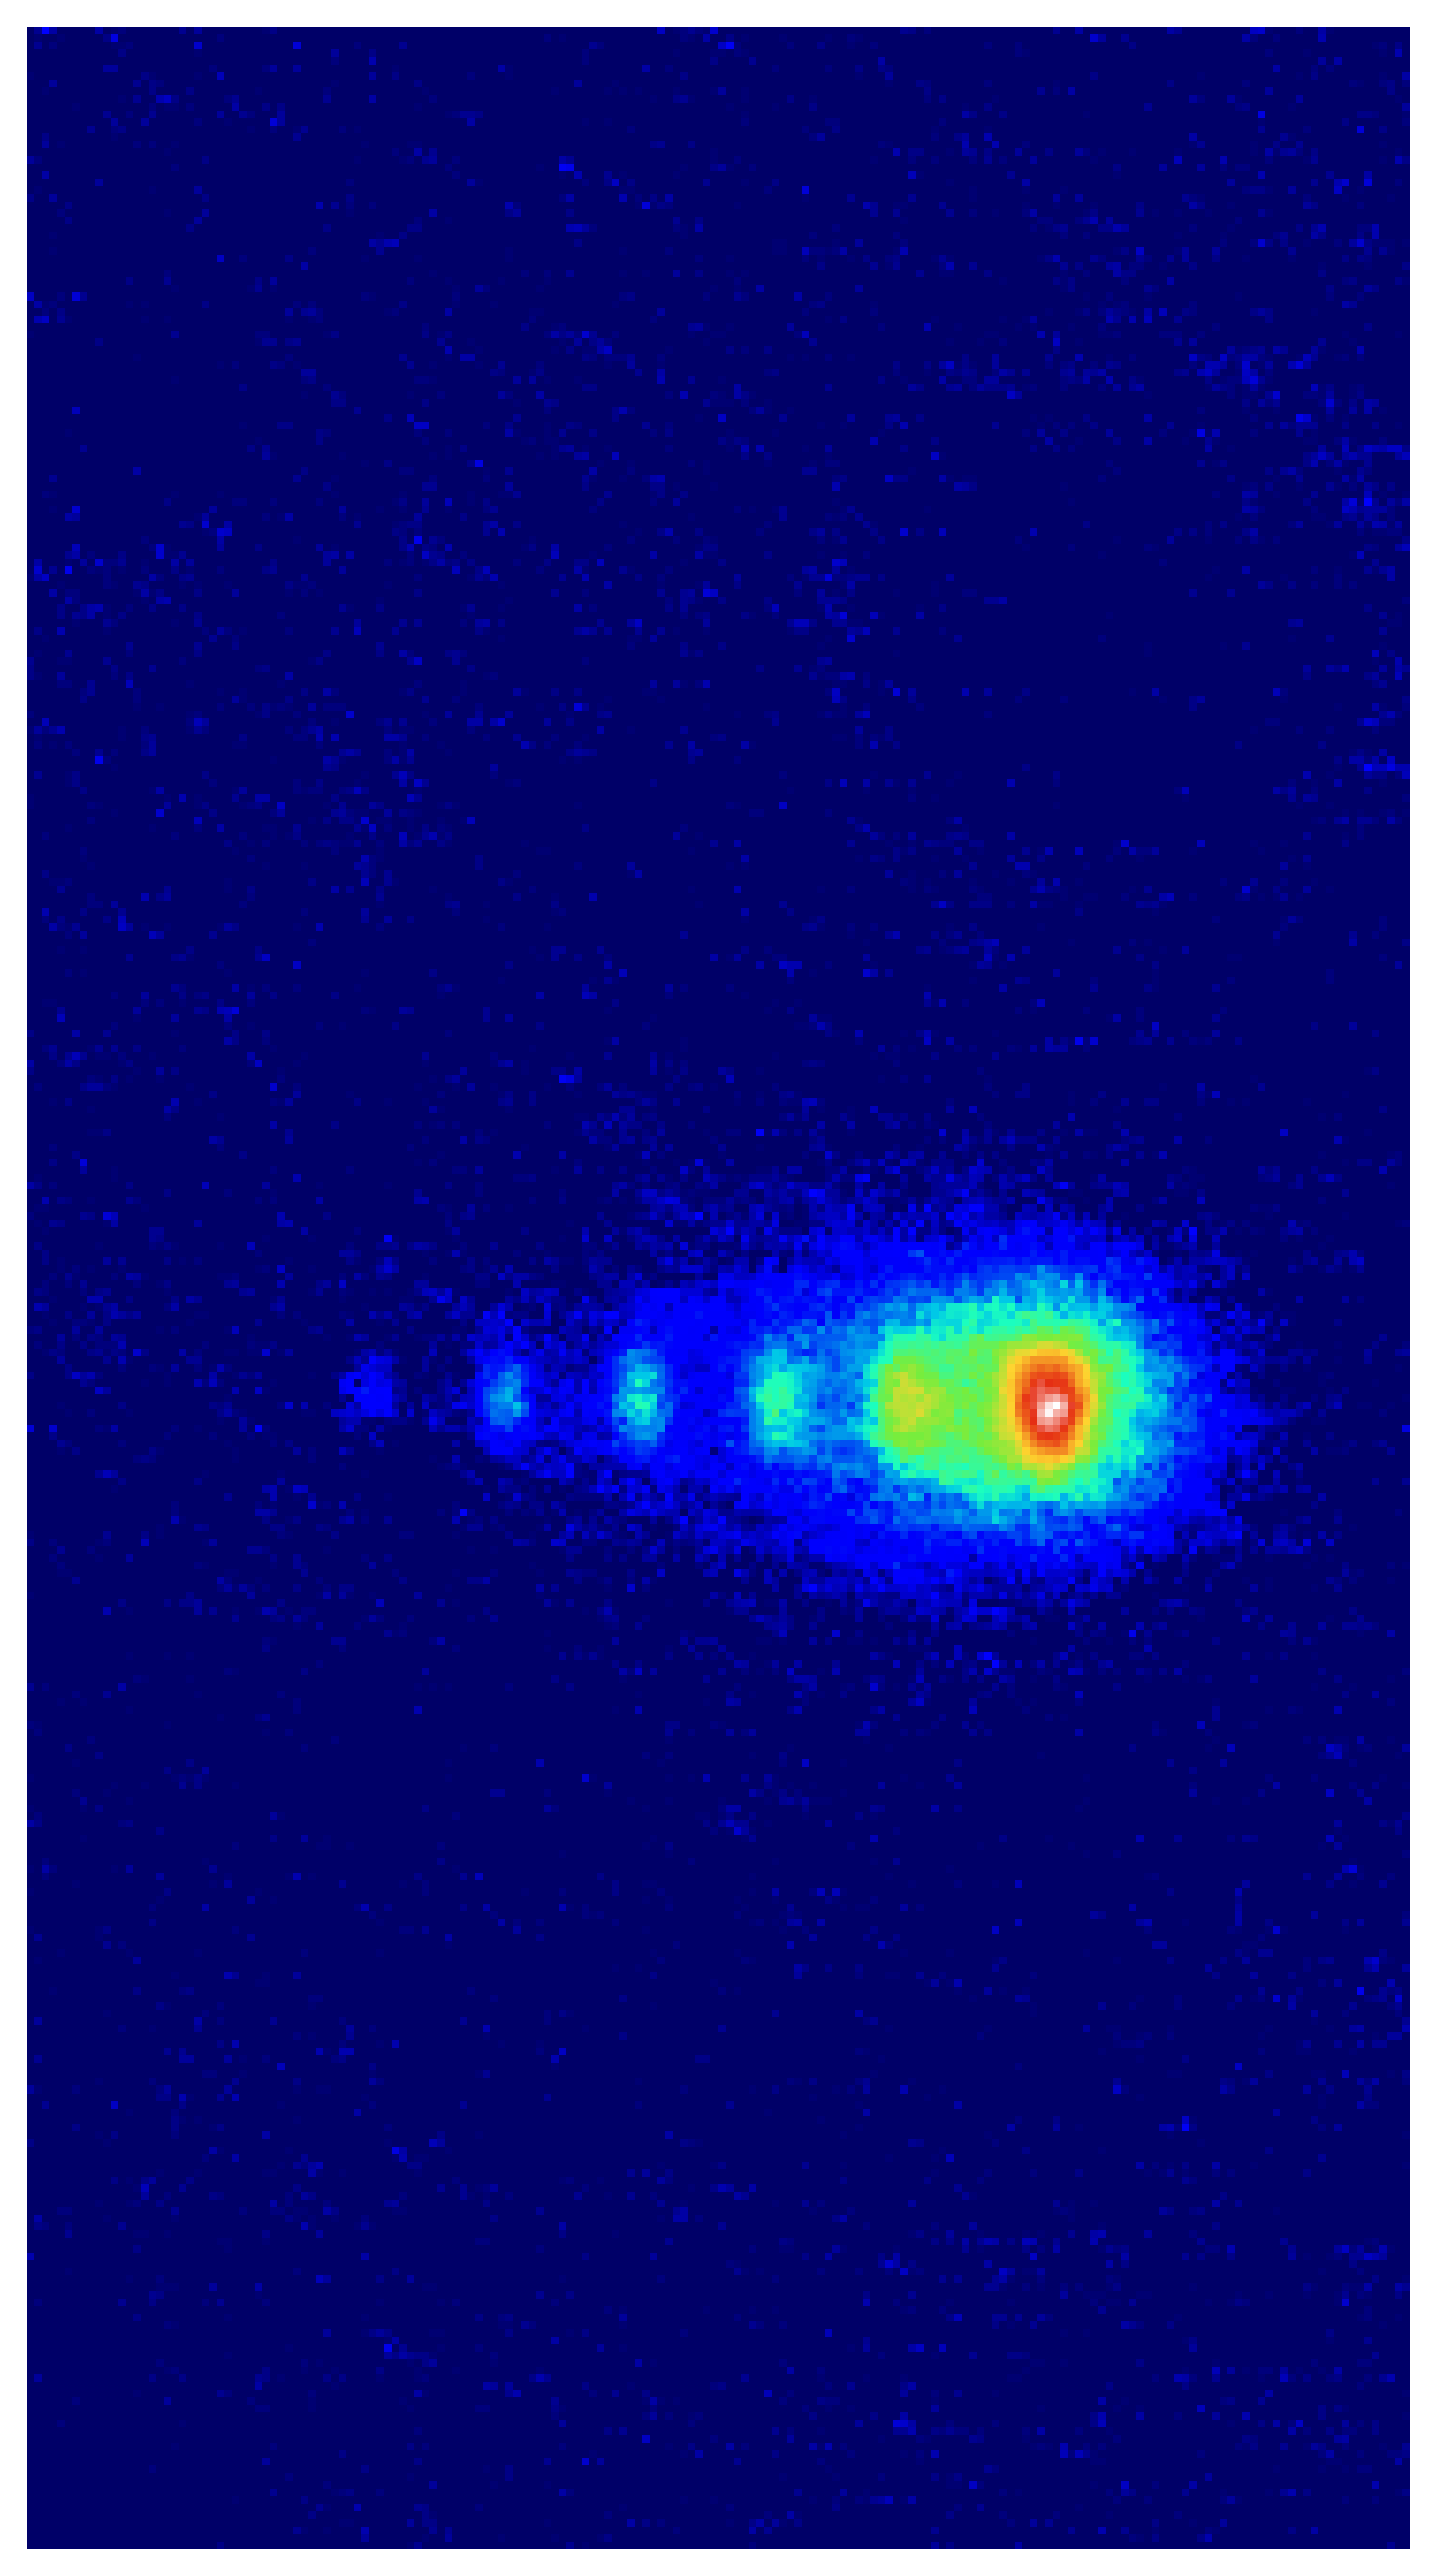
\includegraphics[width=0.7\linewidth]{raman_without_gradient.png}
		\caption{Without magnetic gradient}
		\label{fig:raman_without_gradient}
	\end{subfigure}%
	\begin{subfigure}{.5\textwidth}
		\centering
		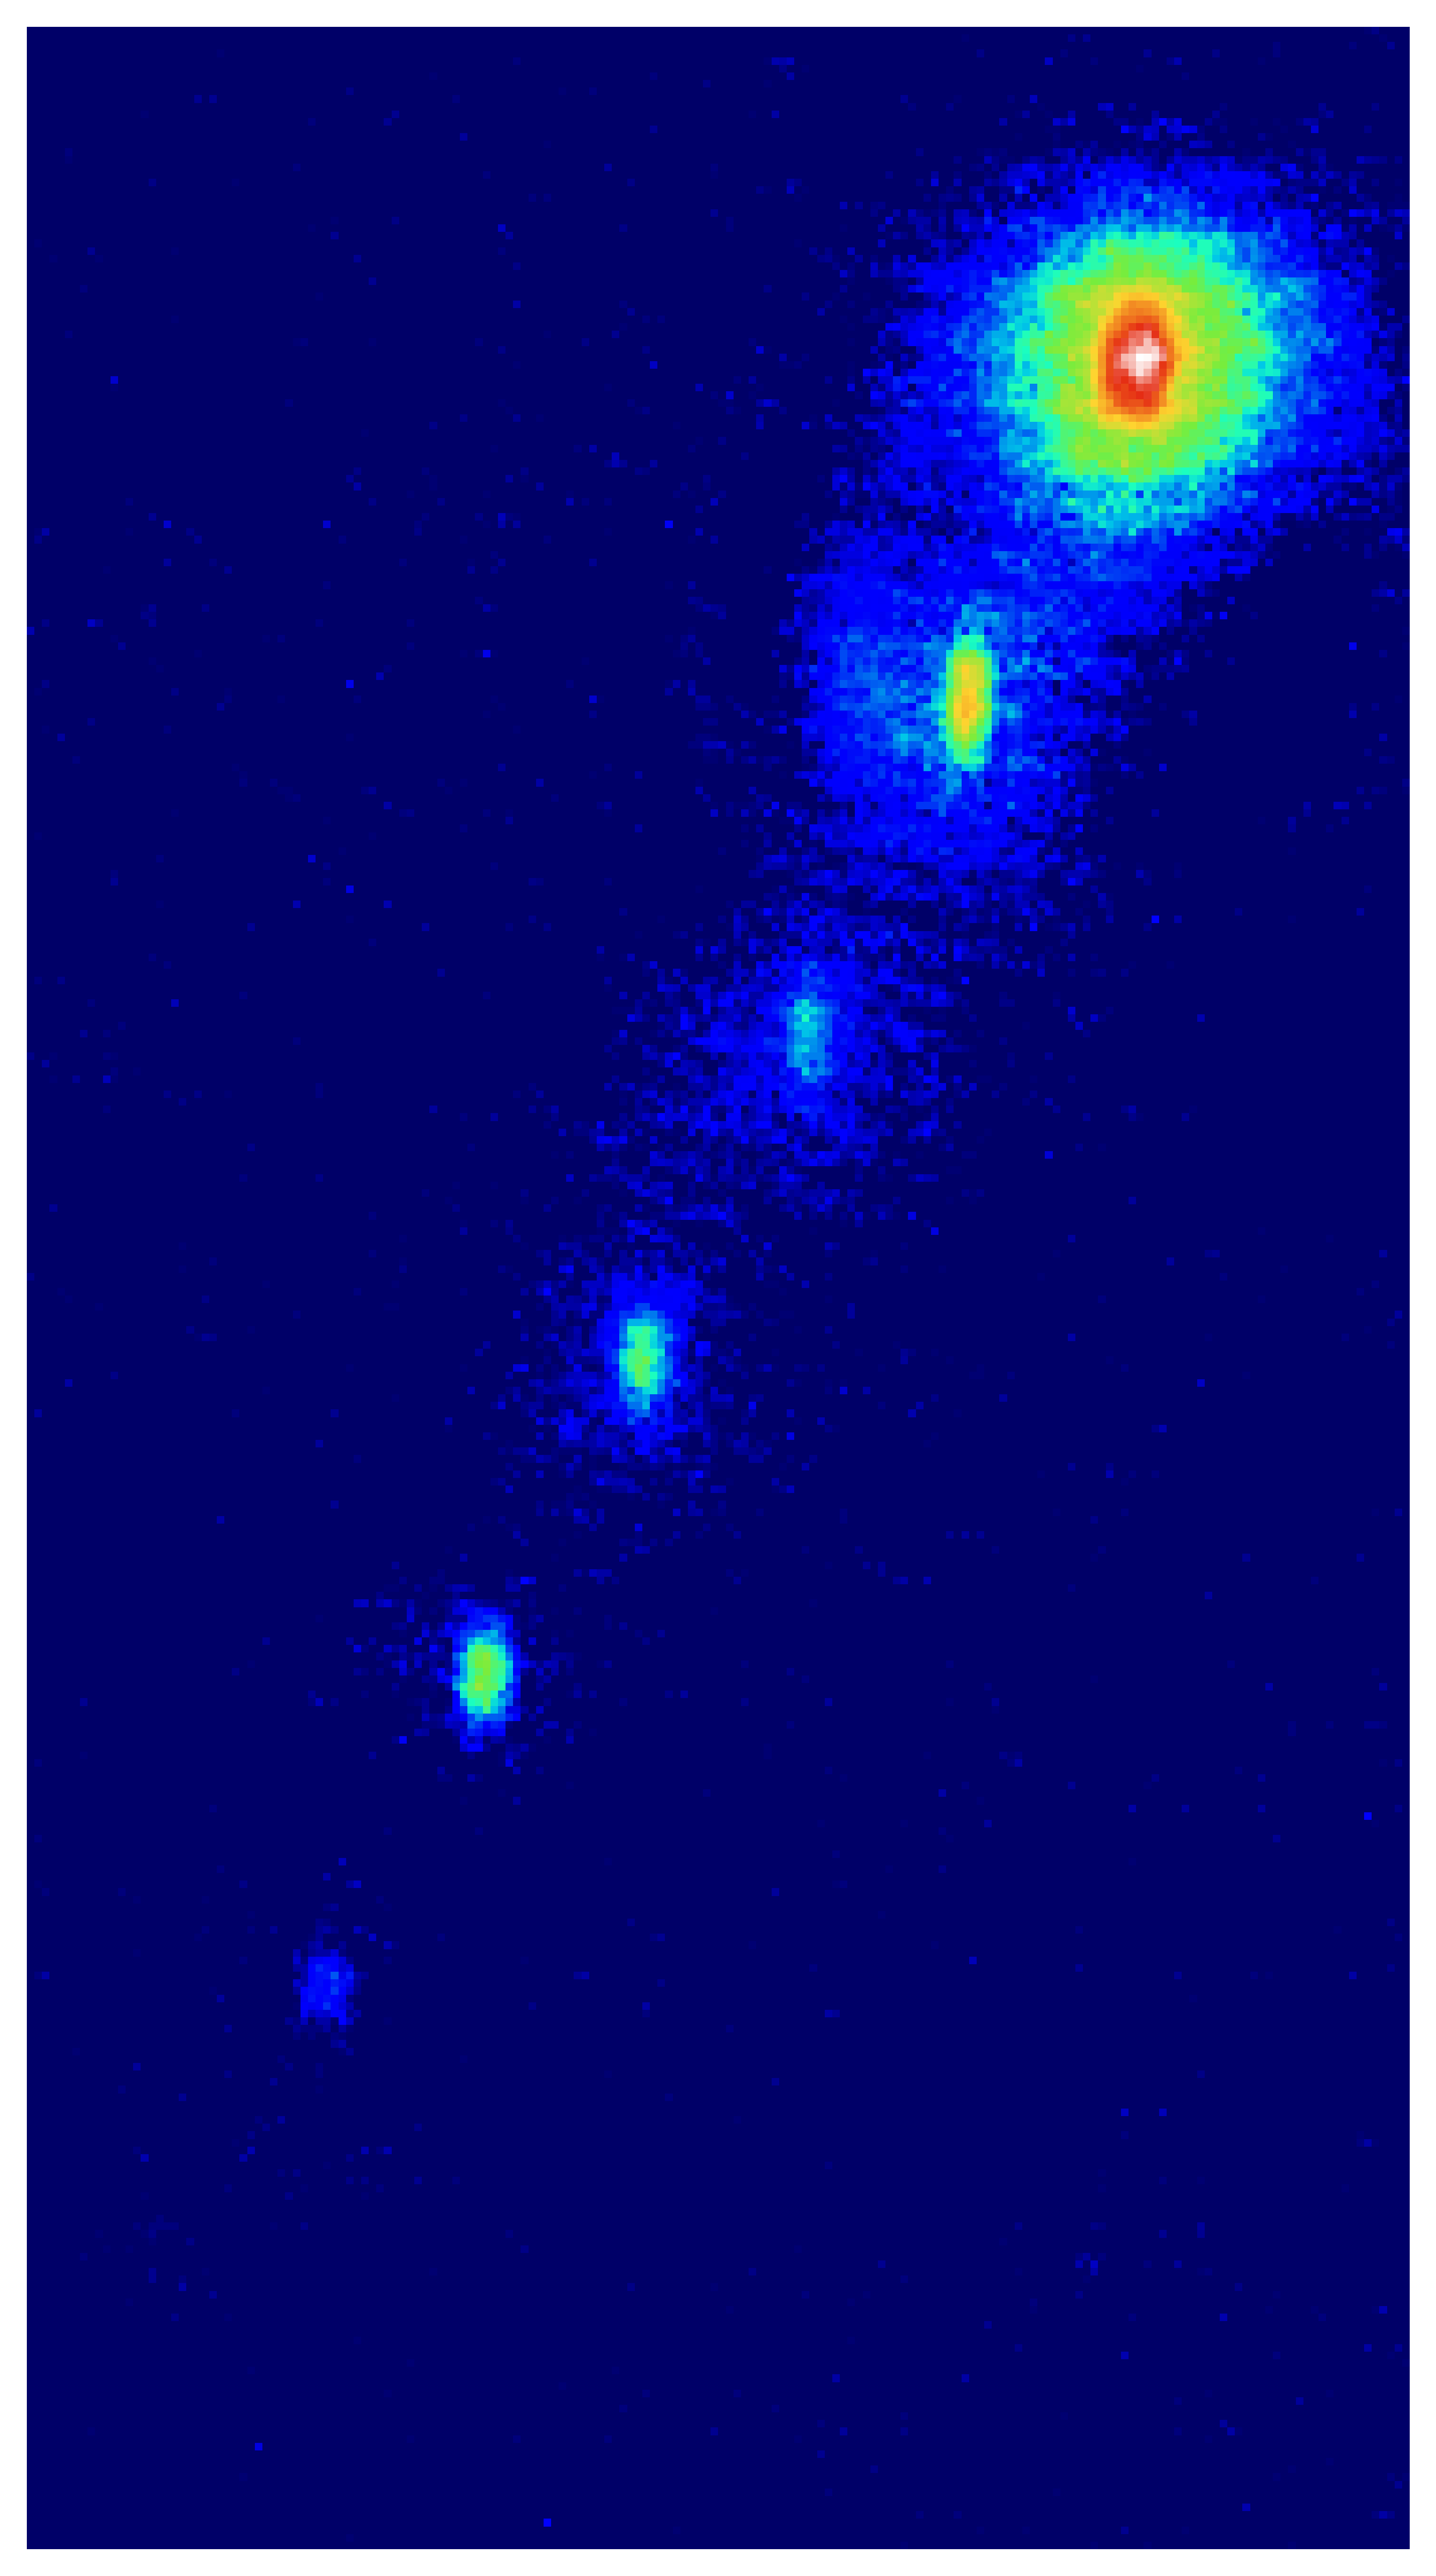
\includegraphics[width=0.7\linewidth]{raman_with_gradient.png}
		\caption{With magnetic gradient}
		\label{fig:raman_with_gradient}
	\end{subfigure}
	\caption[Comparative of two \ac{tof} images following Raman transitions between spin-momentum orders with and without gradient field interaction]{Comparative of two \ac{tof} images following Raman transitions between spin-momentum orders with and without gradient field interaction. This gravitational direction is again matched with the gradient field and corresponds to the left-right axis on both frames. In (b), the Stern-Gerlach force separates the diffracted orders as a function of the spin value $m_J$ throughout the gradient field direction.  }
	\label{fig:raman_gradient}
\end{figure}

%%% Local Variables: 
%%% mode: latex
%%% TeX-master: "Thesis"
%%% End: 
